\documentclass[PM.tex]{subfiles}
\begin{document}
\addtocounter{chapter}{1}
\chapter{Análisis convexo}
\section{Conjuntos convexos}

\begin{defi}
Un conjunto $S\subseteq\R^n$ es \textbf{convexo} si $\forall x^1,x^2\in S$ y $\forall  \lambda\in[0,1]$ se cumple que $\lambda x^1 + (1-\lambda)x^2\in S$.
\end{defi}

\begin{defi}
Un \textbf{semiespacio} es un conjunto de la forma $H^-=\left\{x\in\R^n: a'x\leq b, a\in\R^n, b\in\R\right\}$ o de la forma $H^+=\left\{x\in\R^n: a'x\geq b, a\in\R^n\,b\in\R\right\}$.
\end{defi}

\begin{prop}
$H^-$ es convexo.
\end{prop}

\begin{dem}
Sea $x(\lambda)\equiv \lambda x^1 + (1-\lambda)x^2, \lambda\in[0,1]$. Se tiene lo siguiente
\[
a'x(\lambda)=a'(\lambda x^1 + (1-\lambda)x^2)=\lambda a'x^1 +(1-\lambda)a'x^2\leq \lambda b+(1-\lambda)b=b
\]
Como queríamos demostrar. $\QED$
\end{dem}

\begin{prop}
Si $S_1$ y $S_2$ son convexos entonces $S_1\cap S_2$ es convexo
\end{prop}
\begin{dem}
Definimos $x(\lambda)$ igual que en la demostración anterior. Supongamos que $S_1$ y $S_2$ tienen intersección no vacía, pues en otro caso el resultado se sigue trivialmente. Dados $x^1,x^2\in S_1 \cap S_2$ se tiene por convexidad de $S_1$ que $x(\lambda)\in S_1$. Análogamente, $x(\lambda)\in S_2$. Por lo tanto, $x(\lambda)\in S_1\cap S_2$. $\QED$
\end{dem}

\begin{defi}
Un \textbf{poliedro} es el conjunto de puntos definido por la intersección de un número finito de semiespacios. Visto matricialmente, dados $A\in\R^{m\times n}, b\in \R^n$ se define el poliedro $P=\left\{x\in \R^n: Ax\leq b\right\}$. Si denotamos por $a_i$ a la i-ésima fila de $A$ vemos que este conjunto se reescribe como $\left\{x\in\R^n: a_ix\leq b_i\ \forall i=1,\dots, n\right\}$, que es equivalente a la primera definición. Un poliedro acotado se llama \textbf{politopo}. 
\end{defi}

\begin{coro}
Los poliedros son convexos.
\end{coro}

\begin{defi}
Se define el \textbf{rayo} por un punto $x\in\R^n$ como el conjunto $\left\{y\in\R^n: y=\lambda x, \lambda\geq 0\right\}$.
\end{defi}

\begin{defi}
Sea S convexo y $x\in S$. El punto $x$ dice \textbf{punto extremo} si $x=\lambda x^1 +(1-\lambda)x^2$ con $x^1,x^2\in S$ y $\lambda\in (0,1)$ implica que $x^1=x^2=x$.
\end{defi}
\begin{nota}  En el caso de los poliedros, los puntos extremos coinciden con la idea de vértice. En una bola euclídea cerrada su frontera es de puntos extremos.
\end{nota}

\begin{defi}
Diremos que $d\in\R^n$ es una \textbf{dirección} de $S\subseteq\R^n$ si $\forall x\in S$ se tiene que $x+\alpha d\in S\ \forall\alpha\geq 0$.
\end{defi}

\begin{defi} Una dirección $d$ es \textbf{extrema} si $d=\alpha^1d^1+\alpha^2d^2$, siendo $d^i$ direcciones de $S$ y $\alpha^1,\alpha^2>0$ implica que $d^1$ es proporcional a $d^2$.
\end{defi}

\begin{defi}
Dados $r$ puntos $x^1,\dots, x^r\in\R^n$ llamamos \textbf{combinación convexa} de estos puntos a $\sum_{i=1}^r\lambda_i x^i$ si $\lambda_i\geq 0\ \forall i=1,\dots, r$ y $\sum_{i=1}^r\lambda_i=1$.
\end{defi}

\section{Teorema de Carathéodory}
\begin{defi} Sean $a^1,\dots, a^d\in\R^n$ afínmente independientes (esto es, que fijado un punto, los vectores diferencia de este con los demás son linealmente independientes). Se denomina \textbf{símplex $(d-1)$-dimensional} a 
\[
S(d-1)= \left\{x\in\R^n:x=\sum_{i=1}^d\lambda_i a^i,\lambda_i\geq 0, \sum_{i=1}^d\lambda_i =1\right\}
\]
\end{defi}
\begin{example}
$S(1)$ es un segmento, $S(2)$ es un triángulo relleno y $S(3)$ es un tetraedro relleno.
\end{example}

\begin{defi} Dado un conjunto $S\subset\R^n$, su \textbf{envolvente} (envoltura) \textbf{convexa} $CO(S)$ es
\[
CO(S)=\left\{x\in\R^n: x=\sum_{i=1}^d\lambda_i x^i, d<+\infty, x^i\in S, i=1,\dots, d, \lambda_i\geq 0, \sum_{i=1}^d\lambda_i =1\right\}
\]
$CO(S)$ es el menor convexo que contiene a $S$.
\end{defi}

\begin{defi} Diremos que $C\subset\R^n$ es un cono si contiene a todos sus rayos, es decir, $\forall x\in C$ $\lambda x\in C, \lambda\geq 0$.
\end{defi}
\begin{example}
Una semirrecta que pasa por el origen es un cono. No todos los conos son conjuntos convexos.

\begin{center}
\definecolor{zzttqq}{rgb}{0.6,0.2,0.}
\begin{tikzpicture}[line cap=round,line join=round,>=triangle 45,x=1.0cm,y=1.0cm]
\clip(-3,-2.5) rectangle (3,2.5);
\fill[color=zzttqq,fill=zzttqq,fill opacity=0.10000000149011612] (0.,0.) -- (2.,3.) -- (4.,3.) -- cycle;
\fill[color=zzttqq,fill=zzttqq,fill opacity=0.10000000149011612] (0.,0.) -- (-4.5,-3.) -- (-2.5,-3.) -- cycle;
\fill[color=zzttqq,fill=zzttqq,fill opacity=0.10000000149011612] (0.,0.) -- (4.5,-3.) -- (2.5,-3.) -- cycle;
\draw [color=zzttqq] (0.,0.)-- (2.,3.);
\draw [color=zzttqq] (2.,3.)-- (4.,3.);
\draw [color=zzttqq] (4.,3.)-- (0.,0.);
\draw [color=zzttqq] (0.,0.)-- (-4.5,-3.);
\draw [color=zzttqq] (-4.5,-3.)-- (-2.5,-3.);
\draw [color=zzttqq] (-2.5,-3.)-- (0.,0.);
\draw [color=zzttqq] (0.,0.)-- (4.5,-3.);
\draw [color=zzttqq] (4.5,-3.)-- (2.5,-3.);
\draw [color=zzttqq] (2.5,-3.)-- (0.,0.);
\draw (2.,2.)-- (2.,-2.);
\draw (0.,-4.126140413226097) -- (0.,4.020852846215659);
\draw [domain=-6.367650924229384:10.452891711961001] plot(\x,{(-0.-0.*\x)/2.8572768088505205});
\begin{scriptsize}
\draw [fill=black] (2.,2.) circle (2.5pt);
\draw [fill=black] (2.,-2.) circle (2.5pt);
\end{scriptsize}
\end{tikzpicture}
\end{center}
\end{example}\

\begin{theorem}[Teorema de Carathéodory]
Sea $S\subseteq\R^n$. Si $x\in CO(S)$ entonces:
\[ x = \sum_{i=1}^{n+1} λ_i x^i \]
con $x^i\in S, λ_i ≥ 0$ y $\sum_{i=1}^{n+1}λ_i=1$. Es decir, cualquier punto de la envoltura se puede expresar como combinación lineal convexa de a lo sumo $n+1$ puntos.
\end{theorem}
\begin{dem}
Sea $x \in CO(S)$. Por definición de envoltura convexa, sabemos que $\exists r<+\infty$ tal que:
\[ x = \sum_{i=1}^r λ_i x^i \]
Si $r ≤ n+1$, el teorema está probado. Si $r > n+1$, consideramos los $r-1$ vectores linealmente dependientes $x²-x¹, x³-x¹, \dots, x^{r}-x¹$. Entonces existen $μ_2,\dots,μ_r$ no todos nulos tales que:\[ 0 = \sum_{i=2}^r μ_i (x^i-x¹) = \sum_{i=2}^r μ_i x^i - x^1\sum_{i=2}^r μ_i\]
Tomamos $μ_1 := -\sum_{i=2}^r μ_i$ de manera que se tiene que:
\[ \sum_{i=1}^r μ_i x^i = 0\]
\[ \sum_{i=1}^r μ_i = 0 \]
Sea $α \in \R$. Consideramos:
\[ x = x - α0 = \sum_{i=1}^r λ_i x^i - α \sum_{i=1}^r μ_i x^i = \sum_{i=1}^r (λ_i - α μ_i)x^i \]
Definimos $γ_i = λ_i - α μ_i$ y buscamos $α$ de manera que $γ_i x^i$ sea una combinación convexa. Tomando:
\[ α = \min_{1≤i≤r} \left\{ \frac{λ_i}{μ_i} : μ_i > 0\right\} = \frac{λ_{i*}}{μ_{i*}} \]
Entonces se tiene que $γ_i \geq 0$ y:
\[ \sum_{i=1}^r γ_i = \sum_{i=1}^r (λ_i -α μ_i) = \sum_{i=1}^r λ_i - α \sum_{i=1}^r μ_i = 1 - α \cdot 0 = 1\]
Sin embargo, $γ_{i*} = λ_{i*} - \frac{λ_{i*}}{μ_{i*}}μ_{i*} = 0$, luego $x$ es una combinación convexa de a lo sumo $r-1$ puntos de $S$. Podemos repetir esta construcción hasta llegar a $r = n+1$.
$\QED$
\end{dem}

Consideremos que $||x||$ representa la norma euclídea (se pueden probar resultados análogos con otras normas). 
\begin{theorem}[Teorema de la proyección]
Sea $S\subset\R^n$ convexo y cerrado no vacío, y sea $y\not\in S$ . Entonces existe un único $\overline{x}\in S$ tal que $||y-\overline{x}||=\min_{x\in S}||y-x||$. Además $\overline{x}$ está caracterizado por ser el que verifica $(y-\overline{x})'(x-\overline{x})\leq 0\ \forall x\in S$.

\end{theorem}
\begin{dem}
Veamos que existe $\overline{x}$: consideramos el conjunto \[ \overline{S}=S\cap\{x\in\R^n : ||y-x||\leq ||y-x^0||\}\] para cualquier $x^0\in S$ fijo. Entonces $\inf_{x\in S}||y-x||=\inf_{x\in\overline{S}}||y-x||$. Además, $\overline{S}$ es cerrado y acotado, por tanto el teorema de Weierstrass asegura que existe el $\min_{x\in\overline{S}}||y-x||$ que será $\overline{x}$. Veamos que es único. Supongamos que existe otro $\hat{x}\in S$ tal que 
\[
\gamma=||y-\hat{x}||=||y-\overline{x}||=\min_{x\in\overline{S}}||y-x||
\]
Consideramos el punto medio $\dfrac{\overline{x}+\hat{x}}{2}\in S$ por ser $S$ convexo. Ahora, aplicando la desigualdad triangular
\[
|| y-\frac{\overline{x}+\hat{x}}{2}||=||\frac{y}{2}-\frac{\overline{x}}{2}+\frac{y}{2}-\frac{\hat{x}}{2}||\leq ||\frac{y-\overline{x}}{2}||+||\frac{y-\hat{x}}{2}||=\frac{1}{2}\left(||y-\overline{x}||+||y-\hat{x}||\right)
\]
Como $\gamma$ era la distancia mínima, las desigualdades en realidad son igualdades. La desigualdad triangular solo se convierte en igualdad cuando los vectores son proporcionales, luego $y-\overline{x}=\alpha(y-\hat{x})$, y como ambos tienen norma $\gamma$, necesariamente $|\alpha|=1$. Si $\alpha=-1$ entonces $y-\overline{x}=-(y-\hat{x})\Rightarrow 2y=\hat{x}+\overline{x}\Rightarrow y=\dfrac{\hat{x}+\overline{x}}{2}\in S$, lo cual no es posible porque habíamos supuesto que $y\not\in S$. Por lo tanto $\alpha=1$ y deducimos que $\overline{x}=\hat{x}$.\\
Por último probemos la caracterización. Supongamos que $\overline{x}$ verifica $(y-\overline{x})'(x-\overline{x})\leq 0\ \forall x\in S$. Entonces $\forall x\in S$
\[
||y-x||^2=||y-\overline{x}+\overline{x}-x||^2=||y-\overline{x}||^2+||\overline{x}-x||^2+2(y-\overline{x})'(\overline{x}-x)
\]
El último término es mayor o igual que $0$ por hipótesis, y como la norma es siempre no negativa deducimos que $ ||y-\overline{x}||^2 \leq ||y-x||^2$ $\forall x\in S$. Recíprocamente, supongamos que $\overline{x}$ es el mínimo.  Consideramos entonces para cada $x\in S$ el punto $\overline{x}+\lambda(x-\overline{x})$ con $\lambda\in (0,1)$. Entonces, 
\[
||y-(\overline{x}+\lambda(x-\overline{x}))||^2=||y-\overline{x}||^2+\lambda^2||\overline{x}-x||^2-2\lambda(y-\overline{x})'(x-\overline{x})\geq||y-\overline{x}||.
\]
Restando a ambos lados no queda $\lambda^2||\overline{x}-x||-2\lambda(y-\overline{x})'(x-\overline{x})\geq 0$. Simplificamos usando que $\lambda$ es estrictamente positiva y despejamos y tenemos que $\lambda||x-\overline{x}||\geq 2(y-\overline{x})'(x-\overline{x})$. Como vale para todo $\lambda\in (0,1)$, tomando límite ($\lambda\rightarrow 0$) y deducimos:  $0\geq (y-\overline{x})'(x-\overline{x})$. $\QED$
\end{dem}

\begin{defi} Sean dos conjuntos convexos $S_1,S_2\subset\R^n$ y el hiperplano $H=\{x\in\R^n: p'x=\alpha\}$. Decimos que $H$ separa $S_1$ de $S_2$ si $p'x\leq\alpha$ $\forall x\in S_1$ y $p'x\geq\alpha$ $\forall x\in S_2$. Se dice que $H$ separa estrictamente a $S_1$ de $S_2$ si las desigualdades son estrictas.
\end{defi}

\begin{lema}
Sea $S\subset\R^n$ convexo y cerrado no vacío, sea $y\not\in S$. Existen $p\in\R^n, \alpha\in\R$ tal que $p'y>\alpha$ y $p'x\leq\alpha\ \forall x\in S$.
\end{lema}
\begin{dem}
Por el teorema de la proyección, existe $\overline{x}\in S$ tal que $(y-\overline{x})'(x-\overline{x})\leq 0\ \forall x\in S$. Tomamos $p=(y-\overline{x})$ y $\alpha=p' \overline{x}$. Luego $p'(x-\overline{x})\leq 0\equiv p'x\leq p'\overline{x}$. Además, como $y\not\in S$, $0<||y-\overline{x}||^2=(y-\overline{x})'(y-\overline{x})=p'y-\underbrace{p'\overline{x}}_\alpha \Rightarrow \alpha <p'y$. $\QED$
\end{dem}

\newpage

\begin{lema}[de Farkas]
Sean $A\in \R^{m\times n}, b\in\R^m,x\in\R^n$. Entonces, exactamente uno de los siguientes sistemas tiene solución:
\begin{enumerate}
\item $Ax=b$ con $x\geq 0$ (es decir, todas las componentes de $x$ son no negativas).
\item $u'A\leq 0, u'b>0, u\in \R^m$.
\end{enumerate}
\end{lema}

Antes de demostrarlo vamos a interpretarlo. Sean $a_1,\dots, a_n$ las columnas de $A$. Entonces $Ax=a_1x_1+\cdots +a_nx_n$ con $x_i\geq 0\ \forall i$. Las combinaciones no negativas de los vectores $a_i$ generan un cono. Del segundo sistema $u'a_1\leq 0,\dots , u'a_n\leq 0$. Luego el ángulo que forma $u'$ con cada $a_i$ es mayor de $\frac{\pi}{2}$ y $u$ está en la intersección de todos los hiperplanos. Por otro lado $b$ tiene que formar un ángulo con $u$ menor de $\frac{\pi}{2}$ por lo que estará fuera del cono. Por tanto, si el segundo sistema tiene solución, el primero no puede tenerlo porque en el primero $b$ debe estar dentro del cono. Ver figura.

\begin{dem}\
\begin{enumerate}
\item Supongamos que el primer sistema tiene solución. Es decir, $\exists x^0\mid Ax^0=b, x^0\geq 0$. Por tanto $u'A\cdot x^0\leq 0\equiv u'b\leq 0$, luego no puede haber solución en el segundo.
\item Supongamos que el primer sistema no tiene solución. El conjunto $S=\{v: v=Ax,x\geq 0\}$ es convexo y cerrado en $\R^m$ y $b\not\in S$. Aplicando el lema anterior existen $p\in\R^m,\alpha\in\R$ tal que $p'b>\alpha, p'v\leq\alpha\ \forall v\in S$. Como $0\in S$ deducimos que $p'0\leq\alpha$ luego $\alpha\geq 0$ y por tanto $p'b>\alpha\geq 0\Rightarrow p'b>0$. Ahora tenemos que probar que $p'A\leq 0$. Utilizamos que $p'v\leq\alpha\ \forall v\in S$. Entonces $p'Ax\leq\alpha\ \forall x\geq 0$. De aquí deducimos que todas las componentes de $p'A$ deben ser no positivas, porque si hubiera una componente positiva (supongamos que es la $i$-ésima) entonces $(p'A)_i>0$. Tomando $x_i\rightarrow +\infty$ se tiene que $(p'A)_ix_i\rightarrow +\infty$, por lo que será mayor que $\alpha$.
\[
(p'Ax)=\sum_{j\neq i}(p'A)_jx_j + (p'A)_ix_i \rightarrow +\infty.
\]
Por tanto  $p'A\leq 0$ y hemos encontrado una solución para el segundo sistema.
\end{enumerate}
\end{dem}

\begin{coro}
Los siguientes sistemas son alternativos:
\begin{enumerate}
\item $Ax\geq b, x\geq 0$.
\item $u'A\leq 0, u'b>0, u\geq 0$. 
\end{enumerate}
\end{coro}
\begin{dem}
\begin{enumerate}
\item[]
\item Denotamos por $A_i$ la fila $i$ de $A$ con $i\in\{1,\dots,m\}$. Entonces 
\[
Ax\geq b, x\geq 0 \equiv\begin{cases}
A_1x\geq b_1\equiv A_1x-y_1 & y_1\geq 0\\
\vdots & \\
A_mx\geq b_m\equiv A_mx-y_m & y_m\geq 0\\
x\geq 0 & 
\end{cases}
\]
Es decir, $Ax\geq b, x\geq 0 \equiv Ax-Iy=b, x\geq 0, y\geq 0$, o lo que es lo mismo,
\[(A| -I)\begin{pmatrix}
x\\
y
\end{pmatrix}=b\quad x,y\geq 0.
\]
Ya lo tenemos expresado como el lema de Farkas. Su alternativa es 
\item $u'(A| -I)\leq 0, u'b>0$, es decir, $u'A\leq 0, u'(-I)\leq 0, u'b>0 \Leftrightarrow u'A\leq 0, u\geq 0, u'b>0$. $\QED$
\end{enumerate}
\end{dem}

\begin{lema}
Sea $K\in\R^{n\times m}$ tal que $K'=-K$. Entonces, el sistema $Kx\geq 0, x\geq 0$ tiene una solución que verifica $Kx+x>0$.
\end{lema}
\begin{dem}
Vamos a aplicar el corolario con $b=e_i$ (el vector columna nulo salvo la componente $i$-ésima, que vale $1$), $i=1,\dots, n$.
Consideramos el sistema $Kx\geq e_i, x\geq 0$ o su alternativa $x'K\leq 0, x\geq 0, x'e_i>0$. Sea $\overline{x}^i$ las solución de este par de sistemas en alternativa (es decir, que es solución de uno o de otro). Si $\overline{x}^i$ es solución del primero:
\[
\begin{cases}
K_i\overline{x}^i\geq 1 & \\
K_j\overline{x}^j\geq 0 & j\neq i\\
\overline{x}^i\geq 0 &
\end{cases}
\]
por lo que $K_i\overline{x}^i+\overline{x}^i>0$ y $ K_i\overline{x}^i_i + \overline{x}^i_j\geq 0\ \forall j\neq i$. Por el contrario, si $\overline{x}^i $ es solución del segundo sistema llegamos a que $K'\overline{x}^i\leq 0, \overline{x}^i\geq 0, e'_i\overline{x}^i>0$ y usando que $K$ es antisimétrica obtenemos $K\overline{x}^i\geq 0, e'_i\overline{x}^i>0$. De la última desigualdad deducimos que $\overline{x}^i_i> 0\ \forall i$. Por tanto
\[
K_i\overline{x}^i_i +\overline{x}^i_i>0\quad K_j\overline{x}^i_j +\overline{x}^i_j\geq 0\ \forall j\neq i.
\]
En ambos casos obtenemos lo mismo. Consideramos $\overline{x}=\sum_{i=1}^n\overline{x}^i$. Cumple que $K\overline{x}\geq 0, \overline{x}\geq 0$. Además, 
\[
K\overline{x}+\overline{x}=K(\sum_{i=1}^n\overline{x}^i)+\sum\overline{x}=\sum_{i=1}^n(K\overline{x}^i+\overline{x}^i)>0
\]
$\QED$
\end{dem}

\section{Representación de poliedros}

\begin{defi}
Diremos que un poliedro $P$ está en forma estándar si $P=\{x\in\R^n: Ax=b,x\geq 0\}$ con $A\in\R^{m\times n},$ $b\in\R^m$, $n\geq m$ y $rg(A)=m$.
\end{defi} 
\begin{nota}
Todo poliedro se puede escribir en forma estándar pues $a'x\leq b\equiv a'x+y=b, y\geq 0$ y análogamente restando para la desigualdad contraria.
Si $x_j\in\R$ entonces podemos escribir $x_j=x_j^+ -x_j^-$ siendo $x_j^+=\max{\{x_j,0\}}, x_j^-=-\min{\{x_j,0\}}$.
\end{nota}

Dado que $A\in\R^{m\times n}, b\in\R^m, n\geq m$ y $rg(A)=m$, existe una matriz $B$ de $m$ columas de $A$ que son linealmente independientes, es decir que $rg(B)=m$ ($\exists B^{-1}$). Escribimos entonces $A$ como $[B\ N]$ poniendo las columnas independientes al principio. Las variables del sistema $Ax=b$ también se deben reordenar de modo que 
\[
Ax=b\equiv [B\ N]\begin{bmatrix}
x_B\\
x_N
\end{bmatrix}=b
\]

Sea $A \subset \R^{m \times n}$, $rg(A) = m$, $m ≤ n$ y $b \in \R^m$. Consideramos $P = \{ x \in \R^n : Ax=b, x ≥ 0\}$ (poliedro en forma estándar).

\begin{theorem}[Teorema de caracterización de puntos extremos]\label{carac-extremos}
Sea $P$ un poliedro en las condiciones anteriores. Entonces $x$ es un punto extremo de $P$ si y sólo si existe $B \subset A$ con $B \in \R^{m \times m}$, $rg(B)=m$, $B^{-1}b ≥ 0$ y $x = \begin{pmatrix} B^{-1}b\\0\end{pmatrix}$
\end{theorem}

\begin{dem}
($\Leftarrow$) Supongamos que $x =\begin{pmatrix} B^{-1}b\\0\end{pmatrix}$, $B \subset A$ con $B \in \R^{m \times m}$, $rg(B)=m$, $B^{-1}b ≥ 0$. Usaremos reducción al absurdo, supongamos que existen $x^1$, $x^2 \in P$ tal que $x = λx^1+(1-λ)x^2$ con $λ \in (0,1)$. Tenemos que $A = [B\ N]$ y $x = \begin{pmatrix}x_B\\x_N\end{pmatrix} = \begin{pmatrix} B^{-1}b\\0\end{pmatrix}$, $x^1 = \begin{pmatrix}x_B^1\\x_N^1\end{pmatrix}$ y $x^2 = \begin{pmatrix}x_B^2\\x_N^2\end{pmatrix}$ Luego:
\[ x = \begin{pmatrix} B^{-1}b\\0\end{pmatrix} = λ\begin{pmatrix}x_B^1\\x_N^1\end{pmatrix}+(1-λ)\begin{pmatrix}x_B^2\\x_N^2\end{pmatrix} \]
De ahí, $0 = λ x_N^1 + (1-λ) x_N^2$. Como $x_N^i ≥ 0$, se sigue que $x_N^i = 0$. De $x^i \in P$, se sigue que $Ax^i = b \equiv [B\ N]\begin{bmatrix}x_B^i\\0
\end{bmatrix} = b \equiv Bx_B^i + N0 = b$. Por lo tanto: $x_B^i = B^{-1}b \geq 0$, luego $x^i = \begin{pmatrix}B^{-1}b\\0\end{pmatrix}=x$ para $i=1,2$.


($\Rightarrow$) Supongamos que $x$ fuera un punto extremo de $P$. Se tiene que $Ax=b, x ≥ 0$. Como $rg(A) = m$ podemos suponer sin pérdida de generalidad que $x =(x_1,\dots,x_k,0,\dots,0)$ con $x_i > 0$ y $k ≤ m$.
Vamos a probar que las columnas asociadas a estas coordenadas $(a^1, a^2, \dots, a^k)$ son linealmente independientes. Si no lo fueran, existirían $λ_1,λ_2, \dots, λ_k$ tales que $\sum_{i=1}^k λ_i a^i = 0$. Denotamos or $λ =(λ_1,\dots,λ_k,0,\dots,0)$. Entonces $Aλ=λ_1a^1 + λ_2a^2 + \cdots + λ_ka^k + 0a^{k+1}+\cdots+0a^n = 0$. Entonces podemos considerar los puntos $x^1 = x+αλ$ y $x^2 = x-αλ$ y $α > 0$. Claramente $x^1 \neq x^2$ y $x = \frac{1}{2}x^1+ \frac{1}{2}x^2$. Veamos que $x^i \in P$ para $i=1,2$.
\[ Ax^i = A(x \pm αλ) = Ax \pm α(\underset{=0}{Aλ}) = Ax = b \]
\[ x^i = x \pm αλ = \begin{pmatrix}x_1\\\vdots\\x_k\\0\\\vdots\\0\end{pmatrix} \pm α \begin{pmatrix}λ_1\\\vdots\\λ_k\\0\\\vdots\\0\end{pmatrix} \]
Por hipótesis, $x_1,\dots,x_k > 0$. Tomando $α$ suficientemente pequeño, podemos asegurar que $x_i \pm αλ_i > 0$. Entonces $x^i \geq 0$ y $x^i \in P$. Esto contradice que $x$ sea un punto extremo. Podemos entonces asegurar que $(a^1,\dots,a^k)$ son linealmente independientes. Podemos completar $(a^1,\dots,a^m)$ hasta $m$ columnas linealmente independientes (podemos ya que $rg(A) = m$). Tomamos $B = (a^1,\dots,a^m)$. Entonces:


\[ Ax =[B\ N]\begin{pmatrix}x_1\\\vdots\\x_k\\0\\\vdots\\0\end{pmatrix}_{(n)} = B \begin{pmatrix}x_1\\\vdots\\x_k\\0\\\vdots\\0\end{pmatrix}_{(m)} +N0_{(m-n)} = b \]
Luego: \[ \begin{pmatrix}x_1\\\vdots\\x_k\\0\\\vdots\\0\end{pmatrix} = B^{-1}b \geq 0 \qquad x = \begin{pmatrix}B^{-1}b\\0\end{pmatrix} \]
\end{dem}

\begin{nota}
El número de puntos extremos de los poliedro es finito y está acotado por el número combinatorio $\begin{pmatrix}n\\m\end{pmatrix}$.
\end{nota}

\begin{lema}
$d$ es una dirección de $P$ si y sólo si $Ad=0$, $d ≥ 0$.
\end{lema}

\begin{dem}
$d$ es dirección si y solo si $\forall x \in P$, $x + λd \in P$ $\forall λ ≥ 0$. Equivalentemente, $A(x+λd)= b$ y $x+λd ≥ 0$ $\forall λ ≥ 0$. Esto se cumple si y solo si:
\[ Ax+λAd = b \Leftrightarrow Ad = 0\]
\[ x + λd ≥ 0 \quad \forall λ ≥ 0 \Leftrightarrow d ≥ 0 \]
\end{dem}

\begin{theorem}[Caracterización de direcciones extremas]\label{carac-direcciones}
$d$ es una dirección extrema de $P$ si y solo si $d = \begin{pmatrix}-B^{-1}a_j\\e_j\end{pmatrix}$ donde $B \subset A$, $B \in \R^{m\times m}$, $rg(B) = m$ y $a_j \notin B$ tal que $B^{-1}a_j ≤ 0$. 
\end{theorem}
\begin{dem}
La demostración puede encontrarse en el Bazaraa.
\end{dem}
\begin{nota} El número de direcciones extremas de $P$ es finito y está acotado por $\begin{pmatrix}n\\m\end{pmatrix}(n-m)$.
\end{nota}
\newpage
\begin{theorem}[Teorema de representación de poliedros de Minkowski-Weyl]
Sea $P$ un poliedro en forma estándar y sean $x^1,x²,\dots,x^k$ sus puntos extremos y $d^1,d^2,\dots,d^l$ sus direcciones extremas. Consideramos 
\[ S = \{x \in \R^n : x = \sum_{i=1}^k λ_i x^i + \sum_{j=1}^l μ_j d^j, \sum_{i=1}^k λ_i=1, λ_i ≥ 0, μ_j ≥ 0\ \forall i,j\} \]
Entonces $S = P$. Es decir, cualquier poliedro en forma estándar queda determinado por sus extremos y direcciones extremas.
\end{theorem}

\begin{dem} Lo demostraremos por doble inclusión:
\begin{itemize}
	\item $(S \subseteq P)$ Sea $x \in S$, $x = \sum_{i=1}^k λ_i x^i + \sum_{j=1}^l μ_j d^j$ para algún $λ$ y $μ$.

	\[ Ax = A\left( \sum_{i=1}^k λ_i x^i + \sum_{j=1}^l μ_j d^j\right) =  \sum_{i=1}^k \underset{=b}{λ_i A x^i} + \sum_{j=1}^l μ_j \underset{=0}{Ad^j} = \sum_{j=1}^l b = b \]



	\[ x = \sum_{i=1}^k \underset{≥0}{λ_i} \underset{≥0}{x^i} + \sum_{j=1}^l \underset{≥0}{μ_j}\underset{≥0}{d^j} ≥ 0 \]
	Luego $x \in P$
	
	\item $(P \subseteq S)$ Supongamos que existe $z \in P$ pero $z \notin S$. Como $S$ es un convexo cerrado, existe $p \in \R^n$, $α \in \R$ tales que $p'z > α$, $p'x ≤ α$ $\forall x$ (separación de $z$ y $S$). Tenemos
	\begin{enumerate}
		\item $p'd^j ≤ 0$ $\forall j=1,\dots,l$
		
		Si existiese $j$ tal que $p'd^j > 0$, consideramos el rayo $x + λd^j, λ ≥ 0$ para cualquier $x \in S$, pero entonces $p'(x+λd^j) = p'x + λp'd^j ≤ α$, pero $λp'd^j$ tiende a infinito cuando $λ$ tiende a infinito, luego $p'(x+λd^j)$ no puede estar acotado por ningún $α$.
		\item $p'z > α ≥ p'x^i$ $\forall i=1,\dots,k$
	\end{enumerate}
	Sea $\overline{x}$ el punto extremo tal que $p'\overline{x} = \max_i p'x^i$. Usando el teorema \ref{carac-extremos}: existe una reordenación tal que $\overline{x} = \begin{pmatrix}B^{-1}b\\0\end{pmatrix}$, $A = [B\ N]$, $x = \begin{bmatrix}x_B\\x_n\end{bmatrix}$, $z = \begin{bmatrix}z_B\\z_N\end{bmatrix} \in P$, $Az=b$. De $[B\ N]\begin{bmatrix}z_B\\z_N\end{bmatrix} = b$ obtenemos que $z_B = B^{-1}b-B^{-1}Nz_N$. Luego usando (2):
	\[ 0 < p'(z-\overline{x}) = (p_B'\ p_N') \left[\begin{pmatrix}B^{-1}b-B^{-1}Nz_N\\z_N\end{pmatrix}-\begin{pmatrix}B^{-1}b\\0\end{pmatrix}\right] =-p_B'B^{-1}Nz_N + p'z_N = (p_N'-p_B'B^{-1}N)z_N \]
	Al menos una de las coordenadas de $p_N'-p_B'B^{-1}N$ debe ser positiva. Sea $j$ tal que:
	\[ 0 < (p_N'-P_B'B^{-1}N)_j = p_j - p_B'B^{-1}a_j \]
	Llamemos $y_j\footnote{\url{https://www.youtube.com/watch?v=q6EoRBvdVPQ}} = B^{-1}a_j$ . Veamos que $y_j > 0$. Si $y_j ≤ 0$, $d = \begin{pmatrix}-B^{-1}a_j\\e_j\end{pmatrix}$ debe ser una dirección extrema por el teorema \ref{carac-direcciones}. Entonces $p'd = (p_B'\ p_N')\begin{pmatrix}-B^{-1}a_j\\e_j\end{pmatrix}=-p_B'B^{-1}a_j + p_j > 0$, pero esto contradice (1). Luego $y_j = B^{-1}a_j > 0$. Denotemos por $\overline{b}=B^{-1}b$. Sea $d = \begin{pmatrix}-y_j\\e_j\end{pmatrix}$ y $\hat{x} = \overline{x} + λd$. Veamos que $\hat{x} \in P$ si $λ = \frac{\overline{b}_r}{y_{jr}} = \min\{\frac{\overline{b}_i}{y_{ji}} : y_{ji} > 0\}$..
	\[ A\hat{x} = A\overline{x} + \frac{\overline{b}_r}{y_{r_j}} A d = b + \frac{\overline{b}_r}{y_{jr}} [B\ N] \begin{pmatrix}-B^{-1}a_j\\e_j\end{pmatrix} = b + \frac{\overline{b}_r}{y_{jr}}(-a_j + a_j) = b \]
	Si $i$ es una coordenada de $B$ con $i \neq r$:
	\[ \hat{x}_i = (B^{-1}b)_i + \frac{\overline{b}_r}{y_{jr}}(-y_{ji}) = \overline{b}_i - \frac{\overline{b}_r}{y_{jr}}y_{ji} \]
	Si $y_{ji} < 0 \Rightarrow \hat{x} ≥ 0$ evidentemente. Si $y_{ji} > 0$, entonces $\overline{b}_i - \frac{\overline{b}_r}{y_{jr}}y_{ji} ≥ 0$, ya que $ \frac{\overline{b}_r}{y_{ji}} ≥ \frac{\overline{b}_r}{y_{jr}}$.
	
	Si $i = r$, el resultado es directo, ya que $\overline{b}_r - \frac{\overline{b}_r}{y_{jr}}y_{jr} = 0 ≥ 0$.
	
	Si $i$ es una coordenada que está en $N$, se tiene que $i \neq j$, luego:
	\[ \hat{x}_i = 0 +  \frac{\overline{b}_r}{y_{jr}}0 = 0 \]
	\[ \hat{x}_j = 0 +  \frac{\overline{b}_r}{y_{jr}}1 ≥ 0 \]
	
	Luego $\hat{x} \in P$. Además $\hat{x}$ es un punto extremo representado por las columnas $\hat{B}= (a_1,\dots,a_m)$ y además verifica:
	\[ p'\hat{x} = p'(\overline{x} + \frac{\overline{b}_r}{y_{jr}}d) = p'\overline{x} + \underset{>0}{\frac{\overline{b}_r}{y_{jr}}} \underset{≥0}{p'd} > p'\overline{x} \]
	Esto contradice que $p'\overline{x}$ fuera máximo. Por reducción al absurdo, llegamos a que $z \in S$, lo que acaba la demostración.
	$\QED$
\end{itemize}
\end{dem}

\chapter{Programación Lineal} %Debería ser capítulo 3

\section{Resolución de problemas de Programación Lineal}

Sean $A\in\R^{m\times n},\ rg(A)=m,\ m\leq n,\ b\in\R^m,\ c\in\R^n$. Consideramos el poliedro en forma estándar $P=\{x\in\R^n: Ax=b\}$. El problema de programación lineal consiste en $\underset{x\in P}{\min}\ c'x \equiv \underset{Ax=b,x\geq 0}{\min} c'x\equiv (PL)$. 

\begin{theorem}[Teorema fundamental de la PL] Supongamos que $x^1,\dots ,x^k$ y $d^1,\dots ,d^l$ son respectivamente los puntos extremos y direcciones extremas de $P$. Entonces, la condición necesaria y suficiente para que $(PL)$ tenga solución óptima es que $c'd^j\geq 0\ \forall j=1,\dots, l$. En este caso, una solución óptima siempre se alcanza en un vértice de $P$.
\end{theorem}
\begin{dem}
Planteamos el problema de programación lineal $\underset{Ax=b,x\geq 0}{\min} c'x$. Por el teorema de Weyl, si $x\in P$, podemos escribir $x=\sum_{i=1}^k\lambda_ix^i +\sum_{j=1}^l\mu_j d^j$ con $\lambda_i\geq 0, \mu_j\geq 0, \sum_{i=1}^k\lambda_i=1$. Luego tenemos el problema siguiente
\[\underset{\lambda_i\geq 0, \mu_j\geq 0, \sum_{i=1}^k\lambda_i=1}{\min} c'\left[\sum_{i=1}^k\lambda_ix^i +\sum_{j=1}^l\mu_j d^j\right] \]
Supongamos que $c'd^j\geq 0\ \forall j$. Entonces continuamos la ecuación anterior con 
\begin{gather*}
 \underset{\lambda_i\geq 0, \mu_j\geq 0, \sum_{i=1}^k\lambda_i=1}{\min} \left[\sum_{i=1}^k\lambda_ic'x^i +\sum_{j=1}^l\mu_j \underset{\geq 0}{c'd^j}\right]\geq \underset{\lambda_i\geq 0, \mu_j\geq 0, \sum_{i=1}^k\lambda_i=1}{\min} \left[\sum_{i=1}^k\lambda_ic'x^i\right]\geq \\
\underset{\lambda_i\geq 0, \mu_j\geq 0, \sum_{i=1}^k\lambda_i=1}{\min} \left[\sum_{i=1}^k\lambda_ic'\overline{x}\right]= \underset{\lambda_i\geq 0, \mu_j\geq 0, \sum_{i=1}^k\lambda_i=1}{\min} \left[c'\overline{x}\sum_{i=1}^k\lambda_i\right]=c'\overline{x}
\end{gather*}
donde $\overline{x}$ el punto extremo que minimiza $c'x^i$. Por tanto $c'\overline{x}$ es el valor mínimo, y $\overline{x}$ es un punto extremo. Recíprocamente, si $\exists j\mid c'd^j<0$ consideramos $x\in P$ y el rayo $x+\lambda d^j\in P\ \forall\lambda\geq 0$. 
\[ c'(x+\lambda d^j)=\underset{cte}{c'x} + \underset{<0}{\lambda c' d^j}\underset{\lambda\to\infty}{\longrightarrow} -\infty\]
\end{dem}

\begin{nota}
Dada una función $f$ que alcanza un mínimo en $S\subset\R^n$, entonces \[\min_{x\in S} f(x)= -\max_{x\in S}-f(x)\].
\end{nota}


Supongamos que $\overline{x}$ es un punto extremo de $P$ representado por $B\subset A, rg(B)=m, B^{-1}b\geq 0$. Es decir, $\overline{x}=\begin{pmatrix}
B^{-1}b\\
0
\end{pmatrix}$. Reordenamos las columnas de la forma $A=(B N)$. Sea $x\in P$ otro punto genérico. Entonces $x=\begin{pmatrix}
x_B\\
x_N
\end{pmatrix}$. Como $Ax=b, x\geq 0$ entonces
\[ (B N) \begin{pmatrix}
x_B\\
x_N
\end{pmatrix}= b\equiv Bx_B + Nx_N=b.\]
Luego $x_B=B^{-1}b-B^{-1}Nx_N$, así que 
\[ x=\begin{pmatrix}
B^{-1}b-B^{-1}Nx_N\\
x_N
\end{pmatrix}\]
Ahora bien, \[c'x=(c'_B, c'_N)\begin{pmatrix}
B^{-1}b-B^{-1}Nx_N\\
x_N
\end{pmatrix}=\underbrace{c'_B B^{-1}b}_{c'\overline{x}}-c'_B B^{-1}Nx_N+c'_Nx_N=c'\overline{x}+(c'_N-c'_BB^{-1}N)x_N\]. Si $c'_N-c'_BB^{-1}N\geq 0$, entonces $c'x\geq c'\overline{x}$, por lo que $\overline{x}$ es mínimo. Si esta condición no se cumple, existirá $j$ tal que $a_j\in N$ de forma que $c_j-c'_BB^{-1}a_j<0$. Construimos $d_j=\begin{pmatrix}
-B^{-1}a_j\\
e_j
\end{pmatrix}$ y consideramos $\overline{x}+\lambda d_j,\ \lambda\geq 0$. La evaluación de $x(\lambda)$ será 
\begin{gather*}
c'x(\lambda)=c'(\overline{x}+\lambda d_j)=c'\overline{x}+\lambda c'd_j=c'\overline{x}+\lambda(c'_B, c'_N)\begin{pmatrix}
-B^{-1}a_j\\
e_j
\end{pmatrix}=\\
c'\overline{x}+\lambda\underbrace{(-c'_B B^{-1}a_j +c_j)}_{<0}< c'\overline{x}, \forall\lambda >0.
\end{gather*}
Es decir, $c'x(\lambda)<c'\overline{x}, \forall\lambda >0$. Si $B^{-1}a_j\leq 0$, por el teorema de representación de direcciones extremas, $d_j$ será una dirección de $P$. Por ello, toda la semirrecta $x(\lambda)=\overline{x}+\lambda d_j\subset P$, es decir, $x(\lambda)\in P\forall\lambda >0$. Entonces $c'x(\lambda)\underset{\lambda\to\infty}{\longrightarrow} -\infty$, esto es, no existe mínimo.

En otro caso, $B^{-1}a_j\not\leq 0$. Denotamos $y_j=B^{-1}a_j, \overline{b}=B^{-1}b$. Esto es, $\exists i\mid y_{ij}>0$. Entonces puedo considerar 
\[
\frac{\overline{b}_r}{y_{rj}}=\min\{\frac{\overline{b}_i}{y_{ij}}:y_{ij}>0\}
\]
y el punto $x(\frac{\overline{b}_r}{y_{rj}})=\overline{x}+\frac{\overline{b}_r}{y_{rj}}d_j$. Vamos a probar que $x(\frac{\overline{b}_r}{y_{rj}})\in P$.
\begin{itemize}
\item $x(\frac{\overline{b}_r}{y_{rj}})\geq 0$. Sea $d_j=\begin{pmatrix}
-y_j\\
e_j
\end{pmatrix}$ Si $i\in B, i\neq r$, $\overline{b}_i-\frac{\overline{b}_r}{y_{rj}}y_{ij}\geq 0$ si y solo si $\frac{\overline{b}_i}{y_{ij}}\geq\frac{\overline{b}_r}{y_{rj}}$ si $y_{ij}>0$, lo cual es cierto por definición. Si $y_{ij}<0$ entonces $\overline{b}_i-\frac{\overline{b}_r}{y_{rj}}y_{ij}\geq 0$.\\
Si $r\in B$, $\overline{b}_r-\frac{\overline{b}_r}{y_{rj}}y_{rj}=0$.\\
Si $i\in N, i\neq j$, entonces $\overline{x}_i+\frac{\overline{b}_r}{y_{rj}}d_{ij}$.\\
Si $j\in N$, entonces $\overline{x}_j+\frac{\overline{b}_r}{y_{rj}}d_{ij}=0+\frac{\overline{b}_r}{y_{rj}}\cdot 1=\frac{\overline{b}_r}{y_{rj}}>0$.

\item $Ax(\frac{\overline{b}_r}{y_{rj}})=b$. Comprobémoslo. $Ax(\frac{\overline{b}_r}{y_{rj}})=[B N]\left[\begin{pmatrix}
B^{-1}b\\
0
\end{pmatrix}+\frac{\overline{b}_r}{y_{rj}}\begin{pmatrix}
-B^{-1}a_j\\
e_j
\end{pmatrix}\right]=b+\frac{\overline{b}_r}{y_{rj}}(-a_j+a_j)=b$.
\end{itemize}
En definitiva $x(\frac{\overline{b}_r}{y_{rj}})\in P$ y es un punto extremo con $\hat{B}=B\setminus\{a_r\}\cup\{a_j\}$. Evitando el ciclado (dos soluciones iguales, de forma que alterna de una a otra) este algoritmo encuentra la solución en un número finito de pasos.

\begin{example}
\begin{align*}
\min\ &x_1-3x_2\\
sa & -x_1+2x_2\leq 6\\
   & x_1+x_2\leq 5\\
   &x_1,x_2\geq 0
\end{align*}
Para pasarlo a forma estándar sumamos variables (inmersión de $\R^2$ en $\R^4$).
\begin{align*}
\min\ &x_1-3x_2+0x_3+0x_4\\
sa & -x_1+2x_2+x_3 \quad = 6\\
   & x_1+x_2 \qquad +x_4 = 5\\
   &x_1,x_2,x_3,x_4\geq 0
\end{align*} %alinearlo para que quede todo en su sitio
Entonces $c'=[1,-3,0,0]$, $b=\begin{bmatrix}
6\\
5
\end{bmatrix}$, $A=\begin{bmatrix}
-1 & 2 & 1 & 0\\
1 & 1 & 0 & 1
\end{bmatrix}$. Elegimos las dos últimas columnas de $A$ para construir $B=[a_3\ a_4]$, que tiene inversa. Además cumple que $B^{-1}b=b\geq 0$. El punto es
\[
\begin{bmatrix}
x_3\\
x_4\\
x_1\\
x_2
\end{bmatrix}=\begin{bmatrix}
B^{-1}b\\
0
\end{bmatrix}=\begin{bmatrix}
6\\
5\\
0\\
0
\end{bmatrix}\]
Comprobamos la condición de optimalidad $c'_N-c'_B B^{-1}N\geq 0$. 
\[
[1,-3]-[0,0]I\begin{bmatrix}
-1 & 2\\
1 & 1
\end{bmatrix}=[1,-3]
\]
El coeficiente negativo corresponde a $a_2$. Calculamos $y_2=B^{-1}a_2=I\begin{bmatrix}
2\\
1
\end{bmatrix}\not\leq 0$. Por lo que tenemos que calcular $\min\{\frac{\overline{b}_i}{y_{i2}}:y_{i2}>0\}=\min\{\frac{6}{3},\frac{5}{1}\}=2$. Como este mínimo corresponde al primer elemento del conjunto, se corresponde con la primera columna de $B$, es decir, $a_3$. Por ello, construimos una nueva $B=[a_2\ a_4]=\begin{bmatrix}
2 & 0\\
1 & 1
\end{bmatrix}$ y $B^{-1}=\begin{bmatrix}
\frac{1}{2} & 0\\
-\frac{1}{2} & 1
\end{bmatrix}$. Por tanto $\overline{b}=B^{-1}b=\begin{bmatrix}
3\\
2
\end{bmatrix}\geq 0$. Así pues $\hat{x}=\begin{bmatrix}
x_2\\
x_4\\
x_1\\
x_3
\end{bmatrix}=\begin{bmatrix}
3\\
2\\
0\\
0
\end{bmatrix}$ Ahora, con $N=\begin{bmatrix}
-1 & 1\\
1 & 0
\end{bmatrix}$, $c'_N-c'_B B^{-1}N=[1,0]-[3,0]\begin{bmatrix}
\frac{1}{2} & 0\\
-\frac{1}{2} & 1
\end{bmatrix}\begin{bmatrix}
-1 & 1\\
1 & 0
\end{bmatrix}=[-\frac{1}{2},\frac{3}{2}]$. La coordenada negativa corresponde a $a_1$, que es la candidata para formar la nueva $B$. Tenemos $y_1=B^{-1}a_1=\begin{bmatrix}
\frac{1}{2} & 0\\
-\frac{1}{2} & 1
\end{bmatrix}\begin{bmatrix}
-1\\
1
\end{bmatrix}=\begin{bmatrix}
-\frac{1}{2}\\
\frac{3}{2}
\end{bmatrix}$. Entonces $\min\{\frac{\overline{b}_i}{y_{i1}}:y_{i1}>0\}=\min\{\frac{2}{3/2}\}=\frac{4}{3}$, que corresponde a $x_4$ (segundo elemento de la base), por lo que se elimina $a_4$ de $B$. Resulta la nueva base $B=[a_2\ a_1]=\begin{bmatrix}
2 & -1\\
1 & 1
\end{bmatrix}$. Además,  $N=[a_3\ a_4]=I$, $B^{-1}=\begin{bmatrix}
\frac{1}{3} & \frac{1}{3}\\
-\frac{1}{3} & \frac{2}{3}
\end{bmatrix}$. Así pues,
\[
c'_N-c'_B B^{-1}N=[0,0]-[-3,1]\begin{bmatrix}
\frac{1}{3} & \frac{1}{3}\\
-\frac{1}{3} & \frac{2}{3}
\end{bmatrix}I=[\frac{4}{3},\frac{1}{3}]\geq 0.
\] 
Con lo que hemos encontrado la solución.
\begin{figure}[h!]
	\centering
	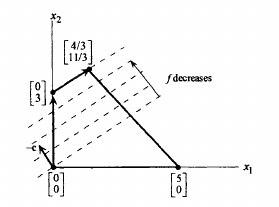
\includegraphics[scale=0.7]{ejemplo}
	\caption{Dibujo del ejemplo}
\end{figure}
\end{example}

\section{Algoritmo del Símplex}
\begin{itemize}
\item Inicialización: encontrar un punto extremo $\overline{x}$ con base $B$.
\item Iteraciones: Calcular $c'_N-c'_B B^{-1}N\equiv c'_N-z_N\equiv \overline{c}_N$. Si este vector es no negativo, paramos(la solución $\overline{x}$ es óptima). En caso contrario, $\exists j\mid c_j-c_B B^{-1}a_j<0$ (si hubiera más de un negativo, elegir el de mayor valor absoluto). Si $y_j=B^{-1}a_j\leq 0$ el problema no tiene mínimo (el mínimo sería $-\infty$). Si $y_{ij}\not\leq 0$ comenzar nuevamente las iteraciones tomando como punto extremo en la inicialización $\hat{x}=\overline{x}+\frac{\overline{b}_r}{y_{rj}}d_j$, siendo $\frac{\overline{b_r}}{y_{rj}}=\min\{\frac{\overline{b_i}}{y_{ij}}:y_{ij}>0\}$, $\overline{b}=B^{-1}b$, $y_j=B^{-1}a_j$, $d_j=\begin{pmatrix}
-y_j\\
e_j
\end{pmatrix}$,
siendo la nueva base la resultante de eliminar la columna $a_r$ de $B$ y en su lugar introducir la columna $a_j$.
\end{itemize}
Este algoritmo tiene el problema de determinar el extremo inicial. Para ello usamos el siguiente método.
\subsection{Método de M-grande}
Consiste en utilizar un problema auxiliar $(P_m)$.
\begin{align*}
 \min\ & c'x+M1^t x_h\qquad \equiv &\min c'x+M\sum_{i=1}^m x_{h_i}\\
&sa:\ Ax+Ix_h=b              & A_1x+ x_{h_1}=b_1 \\
& x\geq 0, x_h\in R^m_+    & \vdots \\
&                          & A_m+ x_{h_m}=b_m
\end{align*}
Donde $A_i$ representa la fila $i$ de la matriz $A$ y $M$ es una constante lo bastante grande (podemos considerar $M=\infty$).  En $P_m$ hay una base obvia $B=[\text{columnas de }x_h]=I$ y $B^{-1}=I\Rightarrow B^{-1}b\geq 0$ si $b\geq 0$. Esto permite aplicar el algoritmo del simplex a $P_m$ para hallar su solución óptima $x^*$. 

Si en $x^*$ hay alguna variable $x^*_{h_i}\neq 0$ para algún $i$, en el objetivo aparece $Mx^*_{h_i}$. Tenemos que $c'x<c'x^*$ para cualquier $x\in P$ (poliedro original), por lo que $P=\emptyset$, porque de haberlo el algoritmo habría encontrado uno más pequeño.  Si $x^*$ es tal que $x^*_h=0$, entonces $x^*$ es solución del problema original $(PL)$. 

\subsection{Forma tabular del algoritmo del símplex}

\begin{align*}
\min & c'x [B N]\\
& Ax=b\\
&x\geq 0
\end{align*}
\begin{tabular}{|c|c| c| c|c|}
\hline
 & & $c'_B$ & $c'_N$ & \\
 \hline
 $x_B$ & $c_B$ & $B$ & $N$ & $b$\\
 \hline

\end{tabular}$\underset{B^{-1},\overline{b}B^{-1}b\geq 0}{\Longrightarrow}$
\begin{tabular}{|c|c| c| c|c|}
\hline
 & & $c'_B$ & $c'_N$ & \\
 \hline
 $x_B$ & $B^{-1}B=I$ & $B^{-1}N=Y$ & $N$ & $\overline{b}$\\
 \hline

\end{tabular}

Apliquemos esto al ejemplo anterior.
\begin{align*}
\min &x_1-3x_2\\
sa & -x_1+2x_2+x_3 \quad = 6\\
   & x_1+x_2 \qquad +x_4 = 5\\
   &x_1,x_2,x_3,x_4\geq 0
\end{align*}
\begin{tabular}{|c|c| c c| c c|c|}

&             &     $c'_N$ & & $c'_B$ & & \\
\hline
 &            & $1$ & $-3$ & $0$ & $0$ & $b$  \\
 \hline
 $x_3$ & $0$ & $-1$ & $2$ &   $1$ &   $0$ & $6$\\
  $x_4$ & $0$ & $1$ & $1$ &    $0$ &  $1$ & $5$\\
 \hline
 &            & $1$ & $\boxed{-3}$ & $0$ & $0$ & Aquí se puede poner $-c_BB^{-1}b$ (objetivo)\\
 \hline
 &             &  $c_N -c_BB^{-1}N$ & & vector $0$& &

\end{tabular}

Hemos señalado el elemento no positivo. \\

Llamamos $N$ y $B$ respectivamente a las matrices cuadradas que se observan.  Llamamos además $y_i$ a los vectores columna ($y_0$ representa los valores de las variables y $y_1$ es la primera columna de $B$). Para conseguir el vector bajo $B$ hacemos $c_B-v_1 B$. Análogamente, para el otro vector hacemos $c_N-v_2 N$. Tenemos que el elemento negativo (en caso de haber más de uno, el más negativo) está bajo $y_2$, que es la segunda columna de la matriz $B$. A partir de eso calculamos $\min\{\frac{6}{2}, \frac{5}{1}\}=3$, es decir, calculamos el mínimo de los $\frac{b_i}{y_i}$ con $i\geq 1$ siempre que $y_i>0$. Este mínimo corresponde a la primera fila de $B$, esto es, a la variable $x_3$. Recordemos que las filas de se asocian a las variables básicas escritas a la izquierda y que las columnas se asocian a las variables colocadas en orden (esto es $y_i\rightarrow x_i$). Ahora nos interesa que la columna $\begin{vmatrix}
1\\
0
\end{vmatrix}$ aparezca en el lugar de la columna $\begin{vmatrix}
2\\
1
\end{vmatrix}$, puesto que $x_2$ se ha convertido por lo anterior en variable básica sustituyendo a $x_3$, y las variables básicas conforman una matriz identidad. Para ello, debemos realizar operaciones por filas. En este caso, basta hacer $\frac{1}{2}F_1$ y a continuación $F_2-F_1$, resultando la tabla siguiente

\begin{tabular}{|c|c| c c| c c|c|}
\hline
 &            & $1$ & $-3$ & $0$ & $0$ & $b$  \\
 \hline
 $x_2$ & $-3$ & $-\frac{1}{2}$ & $1$ &   $\frac{1}{2}$ &   $0$ & $3$\\
  $x_4$ & $0$ & $\frac{3}{2}$ & $0$ &    $-\frac{1}{2}$ &  $1$ & $2$\\
 \hline
 &            & $\boxed{-\frac{1}{2}}$ & $0$ & $\frac{3}{2}$ & $0$ & \\
 \hline

\end{tabular}\

Ahora operamos igual que antes tenemos que el mínimo es $\frac{4}{3}$, y deberíamos seguir así sucesivamente hasta que no quede ningún elemento en la fila inferior que sea negativo.



% Capítulo 4
\chapter{Dualidad en programación lineal}
\section{Introducción}
A cada problema de programación lineal

\begin{center}
\begin{tabular}{cccccc}
(P) & $\min$ & $c_1'x_1$ & $+c_2'x_2$   & $+c_3'x_3$\\
(u') & sa: & $A_{11}x_1$ & $+A_{12}x_2$ & $+ A_{13}x_3$ & $≥ b_1$\\
(v') &     & $A_{21}x_1$ & $+A_{22}x_2$ & $+ A_{23}x_3$ & $≤ b_2$\\
(w') &     & $A_{31}x_1$ & $+A_{32}x_2$ & $+ A_{33}x_3$ & $= b_3$\\
     &     &       $x_1$ &              &               & $≥ 0$\\
     &     &             &      $x_2$   &               & $≤ 0$\\
     &     &             &              &         $x_3$ & libre
\end{tabular}
\end{center}
al que llamaremos primal (P) y donde $x_1, x_2$ y $x_3$ son vectores de variables de decisión, le vamos a asociar otro problema de programación lineal al que llamaremos dual (D) dado por las siguiente transformación:

\begin{center}
\begin{tabular}{cccccc}
(D) & $\max$ & $u'b_1$ & $+v'x_2$ & $+w'x_3$\\
    & sa: & $u'A_{11}$ & $+v'A_{12}$ & $+w'A_{13}$ & $≤ c_1'$\\
    &     & $u'A_{21}$ & $+v'A_{22}$ & $+w'A_{23}$ & $≥ c_2'$\\
    &     & $u'A_{31}$ & $+v'A_{32}$ & $+w'A_{33}$ & $= c_3'$\\
    &     &       $u$  &             &             & $≥ 0$\\
    &     &            &      $v$    &             & $≤ 0$\\
    &     &            &             &      $w$    & libre
\end{tabular}
\end{center}

La transformación que lleva (P) en (D) crea por cada restricción de (P) una variable de decisión en (D) y por cada variable de decisión en (P) una restricción en (D) de a forma que se indica en la siguiente tabla:

\begin{center}
\begin{tabular}{|c|c|}
\hline
	$\min$ & $\max$\\
\hline
	restricción ≥ & variable ≥ 0\\
\hline
	restricción ≤ & variable ≤ 0\\
\hline
	restricción = & variable libre\\
\hline
	variable ≥ 0 & restricción ≤\\
\hline
	variable ≤ 0 & restricción ≥\\
\hline
	variable libre & restricción = \\
\hline
\end{tabular}
\end{center}

\begin{example}
Consideramos el problema
\begin{align*}(P)
	\min c'x\\
	\text{sa:} Ax ≥ b\\
	x ≥ 0
\end{align*}
podemos transformarlo en el problema:
\begin{align*}(P')
	\min c'x + 0x_a\\
	\text{sa:} Ax-Ix_a = b\\
	x, x_a ≥ 0 
\end{align*}
y finalmente pasarlo al problema dual
\begin{align*}(D)
	\max u'b\\
	\text{sa:} u'A ≤ c'\\
	u ≥ 0
\end{align*}
\end{example}

\begin{theorem}[Teorema de dualidad débil]
Para todo $x \in X$ y $u \in U$, donde $X = \{x \in \R^n : Ax ≥ b, x ≥ 0\}$ y $U = \{ u \in \R^m \mid u'A ≤ c', u ≥ 0 \}$, se verifica que $c'x ≥ u'b$.
\end{theorem}

\begin{dem}
$\forall u \in U, \forall x \in X$, se tiene que $u'A ≤ c', x ≥ 0$, luego $u'A x ≤ c'x$. Como $u≥0$ y $Ax≥b$, llegamos a que $u'b ≤ u'Ax ≤ c'x$, lo que demuestra el teorema.
\end{dem}

\begin{obser}
En particular, también se verifica que:
\[ \max\limits_{u \in U} u'b ≤ \min\limits_{x\in X} c'x \]
\end{obser}

\begin{coro}
Si $x^* \in X$ y $u^* \in U$ y $c'x^* = (u^*)'b$, entonces $x^*$ y $u^*$ son soluciones óptimas de (P) y (D) respectivamente.
\end{coro}

\begin{dem}
Por la observación anterior, sigue inmediatamente.
\end{dem}

\begin{theorem}[Teorema de dualidad fuerte]
Si $X \neq \emptyset$ y $U \neq \emptyset$, entonces existen $x^*$ y $u^*$ soluciones óptimas de (P) y (D) respectivamente. Además, $c'x^* = (u^*)'b$.
\end{theorem}

\begin{dem}
Como $U \neq \emptyset$, existe algún punto $\overline{u} \in U$. Entonces $\forall x \in X$, $x'c ≥ \overline{u}'b$. Por tanto (P) no puede decrecer a $-\infty$ y esto indica que debe haber una solución en un punto extremo $x^* \in X$, determinado por una base $B$. Así que:
\[ x^* = \begin{pmatrix}B^{-1} b \\ 0\end{pmatrix}, \qquad B^{-1}b ≥ 0 \]

Veamos ahora que $(u^*)' = c_B'B^{-1}$ es la solución óptima de (D). Es decir, hay que ver que (1) $(u^*)' \in U$ y (2) $(u^*)'b = c'x^*$. Vemos que:
\[ (u^*)'A ≤ c' \equiv (u^*)' (B \ N) ≤ (c_B' \ c_N') \]
Luego:
\[ (u^*)'B ≤ c_B' \equiv c_B'B^{-1}B ≤ c_B' \equiv c_B' ≤ c_B'\]
\[ (u^*)'N ≤ c_N' \equiv c_B'B^{-1}N ≤ c_N' \equiv c_N' - c_B'B^{-1}N ≥ 0\]
Como las ecuaciones del miembro derecho se cumplen, llegamos a que $(u^*)'A ≤ c'$. Por otro lado, dado que $x^*$ es solución óptima de (P) entonces los costes reducidos de las variables asociadas a $x_a$ en $Ax - I x_a = b$ deben ser no negativas. Para cualquier columna $a \in A$ o $-e_j \in -I$, se tiene que:
\[ c_a - c_B' B^{-1} a ≥ 0 \]
\[ c_{e_j} - c_B' B^{-1}(-e_j) ≥ 0 \equiv  -c_B'B^{-1}(-e_j) ≥ 0 \equiv c_B'B^{-1}e_j = (u^*)'e_j ≥ 0 \]
para todo $j$, luego $u^* ≥ 0$, lo que demuestra (1). Por último:
\[ (u^*)'b = c_B'B^{-1}b = \begin{pmatrix}c_B' & c_N'\end{pmatrix}\begin{pmatrix}B^{-1}b\\0\end{pmatrix} = c'x^* \]
\end{dem}

\begin{lema}
El sistema
\begin{equation*}\label{sistema1}\begin{cases}
	Ax - tb ≥ 0\\
	-u'A + tc' ≥ 0\\
	u'b - c'x ≥ 0
\end{cases}\end{equation*}
admite una solución $(x_0,u_0,t_0) ≥ 0$ y verificando
\begin{equation*}\label{sistema2}\begin{cases}
	Ax_0 - t_0b +u_0     > 0\\
	-u'_0A + t_0c' + x_0  > 0\\
	u'_0b - c'x_0 + t_0 > 0
\end{cases}\end{equation*}
\end{lema}

\begin{dem}
Basta ver que la matriz del sistema es antisimétrica:
\[ \begin{pmatrix}
	0  &  A  & -b\\
	-A' &  0  & c\\
	b'& -c'  & 0 
\end{pmatrix}\begin{pmatrix}
	u\\x\\t
\end{pmatrix} ≥ 0 \]
\end{dem}

\begin{theorem}[Teorema de dualidad más fuerte de Gale]
Dados (P) y (D) entonces uno y sólo uno de los siguientes casos son ciertos:
\begin{enumerate}
	\item Ambos problemas tienen soluciones óptimas y sus valores coinciden.
	\item Un problema es infactible y el otro tiene solución ilimitada.
	\item Los dos problemas son infactibles.
\end{enumerate}
\end{theorem}

\begin{dem} Consideramos la solución $(x_0,u_0,t_0)\geq 0$ del sistema del lema anterior. Distinguimos 2 casos:
\begin{enumerate}
	\item $t_0 > 0$. Consideramos $x^* = \frac{x_0}{t_0}$, $u^* = \frac{u_0}{t_0}$ y $t^* = 1$. $(x^*,u^*,t^*)$ sigue siendo solucion del sistema homogéneo. Es decir:
\[\begin{cases}
	Ax^* - b ≥ 0\\
	-(u^*)'A + c' ≥ 0\\
	(u^*)'b - c'x^* ≥ 0
\end{cases}\]
Por lo tanto:
\[\begin{cases}
	Ax^* ≥ b & \Rightarrow x^* \in X\\
	(u^*)'A ≤ c' & \Rightarrow u^* \in U\\
	(u^*)'b ≥ c'x^* & \Rightarrow c'x^* = (u^*)'b
\end{cases}\]
Es decir, $(x^*,u^*)$ es solución óptima de (P) y (D) respectivamente.
	\item $t_0=0$. Se tiene:
\[\begin{cases}
	Ax_0 ≥ 0\\
	-(u_0)'A  ≥ 0\\
	(u_0)'b - c'x^* > 0
\end{cases}\]
	Podemos poner mayor estricto en la última ecuación porque $(u_0)'b-c'x^*+t_0 > 0$.
	\begin{enumerate}
	\item Supongamos que existe $\overline{x} \in X$ y $\overline{u} \in U$, de manera que:
	\[\begin{cases}
		A\overline{x} ≥ b & \overline{x} ≥ 0\\
		\overline{u}'A ≤ c' & \overline{u} ≥ 0
	\end{cases}\]
	\begin{itemize}
	\item Usando que $Ax_0 ≥ 0$ y $\overline{u} ≥ 0$, obtenemos que $\overline{u}'Ax_0≥0$. Si a esto lo sumamos que $\overline{u}'A ≤ c'$, tenemos que $0\leq\overline{u}'Ax_0≤c'x_0 $. En particular $c'x_0 ≥ 0$.
	\item  Usando que $A\overline{x} ≥ b$ y que $u_0 ≥ 0$ deducimos que $u_0'A\overline{x}≥u_0'b $. Por otro lado tenemos que $u'A ≤ 0$ y que $\overline{x} ≥ 0$, luego $0\geq u'A\overline{x}$. Deducimos que $0 \geq u_0'b$.
\end{itemize}
 De estos dos puntos deducimos que $c'x_0  \geq u_0'b$, pero por hipótesis $u_0'b >  c'x^*$ con lo que llegamos a una contradicción.
	\item Supongamos que $\overline{x}$ es solución de $P$ y $U = \emptyset$. Tenemos lo siguiente
	\[ \begin{cases}Ax_0 \geq 0 \\ -u_0'A ≥ 0 \\ u_0'b-c'x_0 > 0 \\  A\overline{x} ≥ b,\overline{x}≥ 0\end{cases} \]
	Vemos que:
	\[ A(\overline{x} + λx_0) = A\overline{x} + λ A x_0 ≥ b \quad \forall λ\geq 0\]
	Como $\overline{x} + λ x_0 ≥ 0$, $\overline{x} + λ x_0 \in X$ para todo $λ > 0$. Además $c'(\overline{x} + λ x_0) = c'\overline{x} + λ c' x_0$ pero veremos que $c'x_0 < 0$.
	\begin{itemize}
	\item Por un lado tenemos que  $u_0'A ≤ 0$ y que $\overline{x} ≥ 0$. Se tiene por tanto que $u_0 A\overline{x} \leq 0$.
	\item Por otro lado, $A \overline{x}\geq b$ y $u_0 \geq 0$, por lo que $u_0'A\overline{x} \geq u_0'b$.
	\end{itemize}
	De estos dos puntos se deduce que $u_0'b\leq 0$, pero de las hipótesis sabemos que $c'x_0 < u_0'b$, luego $c'x_0 <0$. Pero entonces $c'(\overline{x} + λ x_0) \to -\infty$ cuando $λ \to \infty$. Esto es que no puede darse solucion únicamente de un problema y, por descarte, el último caso es que ninguno tenga solución.
	\end{enumerate}
\end{enumerate}
\end{dem}

\begin{theorem}[Teorema de holgura complementaria fuerte]
Si $X \neq \emptyset$ y $U \neq \emptyset$, existen $(\overline{x},\overline{u})$ óptimos de (P) y (D) tales que:
\[ A\overline{x} -b + \overline{u} > 0\]
\[ -\overline{u}A + c' +\overline{x}' > 0\]
\end{theorem}

\begin{dem}
Estamos en el caso 1 del teorema anterior y, por tanto, $t_0 > 0$. Consideramos $\overline{x} = \frac{x_0}{t_0}$, $\overline{u}=\frac{u_0}{t_0}$ y $\overline{t} = 1$. $(\overline{x},\overline{u},\overline{t})$ es solución del sistema \eqref{sistema1} y cumple (evaluando en \eqref{sistema2}):
\[ A\overline{x} -b + \overline{u} > 0\]
\[ -\overline{u}A + c' +\overline{x}' > 0\]
\end{dem}

\begin{theorem}[Otro teorema de holgura complementaria] Sean $x^*$, $u^*$ soluciones factiables de P y D, respectivamente. Entonces $x^*$ y $u^*$ son soluciones óptimas si y sólo si $u^*(Ax^*-b)=0$, $(u'^{*} A-c')x^*=0$.
\end{theorem}
\begin{dem}
\[
\begin{cases}
u'^* A x^* = u'^*b \\
u'^*A x^* = c'x^* 
\end{cases}
\quad c'x^* = u'^*b \Rightarrow \text{$x^*$ es óptima en P y $u^*$ en D}
\]
Recíprocramente, si $c'x^*=u'^*b$. Consideramos el producto, donde cada miembro es $\geq 0$.
\[
u'^*(Ax^*-b)\geq 0
\]
Veamos que $\not >$. Supongamos lo contrario. ($(u^*A) \leq c'$ por ser solución factible del dual):
\[
u'^*Ax^* > u'^* b \Rightarrow c'x^* \geq u'^*Ab>u'^*b
\]
Lo cual es un absurdo. Análogamente deducimos que $(u'^*A-c')x^* \leq 0$. Si la desigualdad fuera estricta llegaríamos al mismo absurdo que en el caso anterior usando que, como $Ax^* \geq b$.
\end{dem}
\section{Análisis de postoptimalidad}
Dado un problema $(P)$ $\min c'x$, $Ax=b$, $x\geq 0$. Considero un vector $d\in\R^n$ y la familia de problemas: $P(\Delta)$: $\min c'x + \Delta d'x$, $Ax=b$, $x\geq 0$. Observemos que $P=P(0)$. Supongamos que B es una base asociada a una solución óptima de $x^*(0)$. Es decir, $x^*(0)=[B^{-1}b | 0]' \geq 0$. Queremos determinar el rango de valores de $\Delta$ que mantienen a $x^*(0)$ como solución óptima de $P(\Delta)$. La condición que certifica que $B$ es una base óptima son:
\begin{itemize}
\item $B^{-1}b \geq 0$.
\item $\overline{c_R}'(0)_N  = \overline{c}'_N = c'_N - c_B'B^{-1}N \geq 0$. 
\end{itemize}
Las condiciones en $P(\Delta)$. 
\begin{itemize}
\item $B^{-1}b \geq 0$.
\item $\overline{c_R}'_N = (c +\Delta d)'_N- (c+\Delta d)'_B B^{-1}N = \overline{c_R}'(0)_N  + \Delta (d_N'-d'_BB^{-1}N) =  \overline{c_R}'(0)_N + \Delta \overline{d}_N\geq 0$. 
\end{itemize}
Para una componente genérica $j\in \mathbb{N}$ se tiene que $\overline{c}_j+\Delta d_j\geq 0$. Entonces:
\[
\begin{cases}
-\frac{\overline{c}_j}{\overline{d}_j} \geq \Delta & si \quad \overline{d}_j <0\\
-\frac{\overline{c}_j}{\overline{d}_j} \leq \Delta & si \quad \overline{d}_j >0
\end{cases}
\Rightarrow \max_{j:\overline{d}_j >0}-\frac{\overline{c}_j}{\overline{d}_j} \leq \Delta \leq \min_{j:\overline{d}_j <0}-\frac{\overline{c}_j}{\overline{d}_j}
\]

\subsection{Análisis de las variaciones en términos independientes}

Sea $z(0)= \min c'x$ sujeto a $Ax=b, x\geq 0$. Queremos estudiar que pasa si elegimos $g\in\R^m$ y construimos el problema
\begin{align*}
z(\Delta)=\min c'x\\
sa: Ax=b+\Delta g\\
\Delta\in\R
\end{align*}
Si $B$ es una base asociada a la solución óptima de $z(0)$, ¿cuál es el rango de $\Delta$ que mantiene $B$ óptima? Las condiciones para que sea óptima son:
\begin{enumerate}
\item Condición de optimalidad. \[\overline{c}_N=c'_N-c'_B B^{-1}N\geq 0.\]
En $z(\Delta)$, teniendo en cuenta que no cambia la función ni las columnas de $A$, esta condición es
\[\overline{c}_N=c'_N-c'_B B^{-1}N\geq 0\] si $\overline{c}_N\geq 0$, que lo es. 
\item Factibilidad. En $z(0)$ es $B^{-1}b=\overline{b}\geq 0$. En $z(\Delta)$ es 
\[B^{-1}b(\Delta)=B^{-1}(b+\Delta  g)=B^{-1}b+\Delta B^{-1}g=\overline{b}+\Delta\overline{g}\geq 0\]
Tomemos un índice $i$ arbitrario.

\[\overline{b}_i+\Delta\overline{g}_i\geq 0\ \forall i=1,\dots, m\Leftrightarrow -\Delta\overline{g}_i\leq\overline{b}_i\]
Si $g_i<0$: $\Delta\leq\frac{\overline{b}_i}{-\overline{g}_i}$.\\
Si $g_i>0$: $\Delta\geq\frac{-\overline{b}_i}{\overline{g}_i}$.\\
Luego
\[\max_{i, g_i>0}\{\frac{-\overline{b}_i}{\overline{g}_i}\}\leq\Delta \leq \min_{i,g_i<0}\{\frac{-\overline{b}_i}{\overline{g}_i}\}\]
\end{enumerate}
\begin{example}
\begin{align*}
\min & -2x_1-x_2 &\\
sa: & x_1+x_2 &\leq 5\\
    & -x_1+x_2 & =0\\
    & 6x_1+2x_2 & \leq 21\\
    & x_1,x_2 & \geq 0
\end{align*}
Pongamos $g'=(0,0,1)$. La báse óptima para $x_1,x_2,x_4$ de este problema era $B=[a_1\ a_2\ a_4]$. Imponemos $B^{-1}(b+\Delta g)\geq 0$ y despejamos $\Delta$ Obtenemos
\[
\begin{pmatrix}
\frac{11}{4}\\
\frac{9}{4}\\
\frac{1}{2}
\end{pmatrix}+\Delta\begin{pmatrix}
\frac{1}{4}\\
\frac{-1}{4}\\
\frac{1}{2}
\end{pmatrix}\geq 0
\]
Por lo tanto $\Delta\in [-1,9]$. Esto quiere decir que $B$ es óptima para $b_3\in[20,30]$. La solución $x(\Delta)=B^{-1}b(\Delta)$ en cada caso será distinta, pero la base será la misma.
\end{example}

\subsection{Añadir una nueva variable $x_{n+1}$ a un problema}
Pasamos del problema $(P)$
\begin{align*}
\min\ & c'x\\
sa:\ & Ax=b\\
 & x\geq 0
\end{align*}
al problema $(P')$
\begin{align*}
\min\ & c'x+c_{n+1}x_{n+1}\\
sa:\ & [A|a_{n+1}]\begin{bmatrix}
x\\
x_{n+1}
\end{bmatrix}=b\\
 &  x,x_{n+1}\geq 0
\end{align*}
Dada $B$ una base óptima en $(P)$ queremos determinar una condición para que sea óptima en $(P')$. Las condiciones para $(P')$ son:
\begin{enumerate}
\item Factibilidad, que es la misma que en $(P)$, $B^{-1}b\geq 0$. 
\item Optimalidad. En $(P)$ \[\overline{c}_N=c'_N-c'_B B^{-1}N\geq 0.\]
En $(P')$
\[\overline{c}_N(P')=(c'_N, c_{n+1})-c'_B B^{-1}[N| a_{n+1}]\geq 0\]
Esto es equivalente a que se cumplan al mismo tiempo
\[\overline{c}_N=c'_N-c'_B B^{-1}N\geq 0,\]
que ya la teníamos, y 
\[c_{n+1}-c'_B B^{-1} a_{n+1}\geq 0.\] Esta sería la condición que buscábamos.

\end{enumerate}

\subsection{Añadir una restricción}
Partimos de nuevo del problema $(P)$ anterior y lo llevamos al problema $(P_q)$
\begin{align*}
\min\ & c'x\\
sa:\  & Ax=b\\
& a'_q x\leq b_q\\
 & x, b_q\geq 0
\end{align*}
Lo escribimos en forma estándar
\begin{align*}
\min\ & c'x\\
sa:\  & Ax=b\\
& a'_q x+h_q= b_q\\
 & x, b_q, h_q\geq 0
\end{align*}
Suponemos que $B$ es una base óptima en $(P)$ y queremos analizar la solución de $(P_q)$. Es decir, $x=\begin{bmatrix}
B^{-1}b\\
0\end{bmatrix}$, $h_q=b_q-(a_q)_B B^{-1}b$.  Evaluamos esta solución en el problema reordenando las columnas de $a_q$.
\[ [(a_q)_B, (a_q)_N]\begin{bmatrix}
B^{-1}b\\
0\end{bmatrix} +h_q=b_q.\] Hay que comprobar que $h_q\geq 0$ para que tenga sentido. La base asociada a esta solución es
\[ B_q=\begin{bmatrix}
B & 0\\
(a_q)_B & 1
\end{bmatrix}.\] La última columna proviene de haber añadido $h_q$. Su inversa tiene la siguiente forma:
\[ B_q^{-1}=\begin{bmatrix}
B^{-1} & 0\\
\alpha & 1
\end{bmatrix},\] con $\alpha$ tal que $(a'_q)_B B^{-1} +\alpha=0$. Es decir, $\alpha=-(a'_q)_B B^{-1}$. Queda pues, finalmente así la inversa (comprobarlo)
\[ B_q^{-1}=\begin{bmatrix}
B^{-1} & 0\\
-(a'_q)_B B^{-1} & 1
\end{bmatrix}.\]
Para que esta solución sea óptima 
\begin{enumerate}
\item $B_q^{-1}\begin{bmatrix}
b\\
b_q
\end{bmatrix}\geq 0$. Esto es equivalente a $\begin{bmatrix}
B^{-1} & 0\\
-(a'_q)_B B^{-1} & 1
\end{bmatrix}\begin{bmatrix}
b\\
b_q
\end{bmatrix}=\begin{bmatrix}
B^{-1}b\\
-(a'_q)_B B^{-1}+b_q
\end{bmatrix}\geq 0$. Observamos que la única condición nueva es $-(a'_q)_B B^{-1}+b_q\geq 0$.
\item $\overline{c}_N(P_q)=c'_N-(c'_B,0)B_q^{-1}\begin{bmatrix}
N\\
(a'_q)_N
\end{bmatrix}\geq 0$. Esto es equivalente a $c'_N-[c'_B B_q^{-1} N + 0]=\overline{c}_N\geq 0$.
\end{enumerate}

\begin{example}
Añadimos al ejemplo anterior la restricción $x_1+x_2\leq 4$ y lo escribimos en forma estándar añadiendo $x_3,x_4,x_5,x_6$.
\begin{align*}
\min & -2x_1-x_2 &\\
sa: & x_1+x_2 +x_3 &= 5\\
    & -x_1+x_2 +x_4 & =0\\
    & 6x_1+2x_2  +x_4 & = 21\\
    & x_1+x_2 +x_6  & = 4\\
    & x_1,x_2,x_3,x_4,x_5,x_6 & \geq 0
\end{align*}
Obsérvese que hemos añadido $x_4$ aunque ya teníamos una igualdad en la segunda restricción. Esto no importa porque la solución puede dar $x_4=0$. En este problema $a'_q=(1,1,0,0,0)$, $b_q=4$ y $B_6=[a_1\ a_2\ a_4\ a_6]$ (la de antes añadiendo $a_6$). Para que sea óptima $-(a'_q)_B B^{-1}+b_q\geq 0$. Si operamos nos da $-\frac{13}{4}\not\geq 0$, por lo que no es óptima. Tendríamos entonces
\[ B_q^{-1}\begin{bmatrix}
5\\
0\\
21\\
4
\end{bmatrix}=\begin{bmatrix}
\frac{11}{4}\\
\frac{9}{4}\\
\frac{1}{2	}\\
-\frac{13}{4}
\end{bmatrix}\]
Como tenemos un elemento negativo, usaríamos el método del símplex dual.
\end{example}

\section{Precios Sombra}
Definimos 
\begin{align*}
f:\R^m\longrightarrow \R & & &\\
 f(b) = & \min\ & c'x\\
                                &sa:\  & Ax=b\\
       							& & x\geq 0
\end{align*}
Queremos derivar esta función. Supongamos en este problema que las bases factibles son $B_1,\dots, B_r$. Consideramos el problema dual que verifica
\begin{align*}
 f(b) = & \min\ & c'x\quad  & =\max\ u'b \quad  = \max\{c'_{B_1}B_1^{-1}b,\dots, c'_{B_r}B_r^{-1}b\}\\
        &sa:\   Ax=b       &sa:\ & u'A\leq c\\
        &  x\geq 0         & & u\in\R^m 
\end{align*}
Llamamos $u_i=c'_{B_i}B_i^{-1}$. Entonces, $f(b)=\max_{1\leq i\leq r}u_i'b=u'_k b$. Ahora derivamos
\[\frac{\partial f}{\partial b_i}=\frac{\partial }{\partial b_i}\left(\sum_{j=1}^m u_{kj}b_j\right)=u_{ki}\]
Hemos llegado a la solución óptima del dual en su variable $i$-ésima. 
\begin{example}
$g'=(0,0,1)=e'_3$. Teníamos que $z(\Delta)$ al variar $b_3\in [20,30]$ mantiene la base óptima.
\begin{gather*}
f(\Delta)= z(\Delta)=c'_B B^{-1}b(\Delta)=c'_B B^{-1}(b+\Delta e_3)=\\
c'_B B^{-1} b +\Delta c'_B B^{-1} e_3 =\frac{31}{4}-\frac{1}{4}\Delta
\end{gather*}
Luego $\frac{\partial z}{\partial\Delta}=-\frac{1}{4}$. Si quisiéramos utilizar el resultado anterior, tendríamos que obtener la solución óptima y multiplicar por $e_3$ (quedarnos con la tercera componente). La solución óptima del dual es
\[(u^*)'=c'_B B^{-1}=[-2\ -1\ 0]B^{-1}=[-\frac{1}{2}\ 0\ -\frac{1}{4}]\]
Por lo tanto. $\frac{\partial z}{\partial\Delta}=\frac{\partial z}{\partial b_3}=u^*_3=-\frac{1}{4}$.
\end{example}
\newpage
\section{Resumen}
Condiciones para el análisis de postóptimalidad
\begin{itemize}
\item En la función objetivo
\[
\max_{j:\overline{d}_j >0}-\frac{\overline{c}_j}{\overline{d}_j} \leq \Delta \leq \min_{j:\overline{d}_j <0}-\frac{\overline{c}_j}{\overline{d}_j}
\]
\item En el término independiente
\[\max_{i, g_i>0}\{\frac{-\overline{b}_i}{\overline{g}_i}\}\leq\Delta \leq \min_{i,g_i<0}\{\frac{-\overline{b}_i}{\overline{g}_i}\}\]
\item Añadir una nueva variable
\[c_{n+1}-c'_B B^{-1} a_{n+1}\geq 0.\]
\item Añadir una nueva restricción
\[-(a'_q)_B B^{-1}+b_q\geq 0\]
\end{itemize}
{\large\bf LOGIC INTERLUDE}
\begin{theorem}
Si $c \in Res(c_1,c_2)$ entonces $\{ c_1, c_2 \} \models c$.
\end{theorem}

\begin{dem}

Sea $I \models \{ c_1, c_2\}$. Hay que demostrar que $I \models c$. Como $c \in Res(c_1,c_2)$, entonces existe $L \in c_1$ tal que $c = Res_L(c_1, c_2) = (c_1-\{ L \} \cup (c_2 - \{ L^c \})$.

Consideramos dos casos:
\begin{itemize}
	\item Si $I(L) = 1$, entonces $I(L^C)=0$. Por otro lado, sabemos que $I$ es modelo de $c_2$, luego existe $L' \in C_2$ tal que $I(L')=1$. De $I(L^C)=0$ y $I(L')=1$, tenemos que $L^C \neq L'$. Luego $L' \in c_2 - \{ L ^C \}$. Luego $L' \in c$. Por lo tanto, $I \models c$.
	\item $I(L) = 0$. Como $I \models c_1$, existe $L' \in c_1$ tal que $I(L') = 1$. Entonces $L' \neq L$, luego $L' \in c_1 - \{ L \}$. Entonces $L' \in c$ y $I \models c$. 
\end{itemize}
\end{dem}

% Tema 5
\chapter{Programación Lineal Entera}

\section{Poliedros enteros y matrices totalmente unimodulares}
Consideramos el problema

\begin{align*}
(PE) & \min c'x\\
	 & A x = b\\
	 & x \in \mathbb{Z}_+^n\\
	 & A \in \R^{m \times n}, b \in \R^m, c \in \R^n
\end{align*}

Denotaremos por $z_{PE}$ al valor óptimo de este problema. PE tiene asociado otro problema que denominaremos el ``problema relajado lineal'' y denotamos por (LP) que consiste;

\begin{align*}
(LP) & \min c'x\\
	 & A x = b\\
	 & x \in \mathbb{R}_+^n
\end{align*}

\begin{obser}
Si $x$ es factible en $PE$ entonces también lo es en $LP$.
\[ \{x \in \mathbb{Z}_+^n : Ax=b \} \subset \{x \in \mathbb{R}_+^n : Ax=b \} \]

Esto implica que $z_{LP} ≤ z_{PE}$, donde $z_{LP} $ es el valor óptimo de $LP$.
\end{obser}
\begin{defi}
Un problema es de \textbf{programación binaria} ó $\{0,1\}$ si sus variables están restringidas a tomar valores en $\{0,1\}$.
\end{defi}
\newpage
\begin{defi}
Decimos que un problema es entero-mixto $(PME)$ si:

\begin{align*}
(PME) & \min c'x+d'y\\
	  & A_1 x + A_2 y = b\\
	  & x \in \Z_+^{n_1}, y \in \R_+^{n_2}\\
	  & A_1 \in \R^{m\times n_1}, A_2 \in \R^{m \times n_2}, b \in \R^m, c \in \R^{n_1}, d \in \R^{n_2}
\end{align*}
\end{defi}
\begin{example}
Veamos que no siempre coincide $z_{PE}$ con un redondeo de $z_{LP}$.

\begin{align*}
(PME) & \min 21x_1+11x_2\\
	  & 6x_1+4x_2 ≤ 13\\
	  & x_1,x_2 \in \Z_+\\
(LP) & x_1,x_2 \in \R_+
\end{align*}

La solución óptima de $LP$ es $(\frac{13}{7},0)$. El redondeo más cercano es $(2,0)$. El redondeo por abajo es $(1,0)$. Ninguno es la solución óptima, que es $(0,3)$, como se puede comprobar evaluando la función en cada uno de los puntos de coordenadas enteras señalados en la figura.

\begin{center}
\definecolor{qqqqff}{rgb}{0.,0.,1.}
\definecolor{zzttqq}{rgb}{0.6,0.2,0.}
\definecolor{uuuuuu}{rgb}{0.26666666666666666,0.26666666666666666,0.26666666666666666}
\definecolor{cqcqcq}{rgb}{0.7529411764705882,0.7529411764705882,0.7529411764705882}
\begin{tikzpicture}[line cap=round,line join=round,>=triangle 45,x=1.0cm,y=1.0cm]
\draw [color=cqcqcq,, xstep=1.0cm,ystep=1.0cm] (-4.3,-1.3) grid (5.3,4.3);
\draw[color=black] (-4,0.) -- (5,0.);
\foreach \x in {-4,-3.,-2.,-1.,1.,2.,3.,4.,5.}
\draw[shift={(\x,0)},color=black] (0pt,2pt) -- (0pt,-2pt) node[below] {\footnotesize $\x$};
\draw[color=black] (0.,-1.) -- (0.,4.752470459668063);
\foreach \y in {-1.,1.,2.,3.,4.}
\draw[shift={(0,\y)},color=black] (2pt,0pt) -- (-2pt,0pt) node[left] {\footnotesize $\y$};
\draw[color=black] (0pt,-10pt) node[right] {\footnotesize $0$};
\clip(-3.969088632379392,-1.385270587163902) rectangle (8.703087676160555,4.752470459668063);
\fill[color=zzttqq,fill=zzttqq,fill opacity=0.10000000149011612] (0.,3.25) -- (0.,0.) -- (2.1666666666666665,0.) -- cycle;
\draw [domain=-3.969088632379392:8.703087676160555] plot(\x,{(--13.-6.*\x)/4.});
\draw [color=zzttqq] (0.,3.25)-- (0.,0.);
\draw [color=zzttqq] (0.,0.)-- (2.1666666666666665,0.);
\draw [color=zzttqq] (2.1666666666666665,0.)-- (0.,3.25);
\draw [dash pattern=on 3pt off 3pt,domain=-3.969088632379392:8.703087676160555] plot(\x,{(--46.-21.*\x)/11.});
\begin{scriptsize}
\draw [fill=uuuuuu] (0.,3.25) circle (1.5pt);
\draw [fill=uuuuuu] (0.,0.) circle (1.5pt);
\draw [fill=uuuuuu] (2.1666666666666665,0.) circle (1.5pt);
\draw [fill=qqqqff] (0.,3.) circle (2.5pt);
\draw [fill=qqqqff] (0.,2.) circle (2.5pt);
\draw [fill=qqqqff] (0.,1.) circle (2.5pt);
\draw [fill=qqqqff] (1.,0.) circle (2.5pt);
\draw [fill=qqqqff] (2.,0.) circle (2.5pt);
\draw [fill=qqqqff] (1.,1.) circle (2.5pt);
\end{scriptsize}
\end{tikzpicture}
\end{center}

\end{example}

\begin{obser}
La solución óptima del $PME$ coincide con la solución del problema de optimización:
\[
\begin{aligned}
& \min
& & c'x \\
& \text{sujeto a}
& & x \in conv\{x \in \R^n : Ax=b, x \in x \in \Z_+^n\}
\end{aligned}
\]
Sin embargo, calcular la envolvente convexa se puede volver muy costoso en dimensiones superiores.
\end{obser}

\begin{example}[Problema de la mochila]
Un conjunto de productos numerados de $1$ a $n$. El producto $i$ ocupa un volumen $a_i$ y reporta una satisfacción $p_i$. Dada una mochila con capacidad $V$ determinar la carga que maximiza la satisfacción. Definimos las variables $x_i$ con $x_i = 1$ si decido incluir el producto $i$ y $x_i = 0$ en caso contrario. Podemos definir el problema binario:
\[
\begin{aligned}
& \max
& & \sum_{i=1}^n p_i x_i \\
& \text{sujeto a}
& & \sum_{i=1}^n a_i x_i ≤ V\\
& & & x_i \in \{0,1\}\ \forall i 
\end{aligned}
\]
\end{example}

\begin{example}[Problema de transporte]
Consideramos $m$ puntos de suministro y $n$ puntos de consumo. Cada punto de suministro $i$ dispone de una oferta $o_i$ con $i = 1,\dots,m$. Cada punto de consumo $j$ tiene una demanda $d_j$ con $j = 1,\dots,n$. Supongamos que $o_i,d_j \in \Z_+\ \forall i,j$ porque lo que distribuye son productos indivisibles. Además, $\sum_{i=1}^m o_i = \sum_{j=1}^m d_j$. El coste unitario de enviar una unidad desde $i$ a $j$ es $c_{ij}$. El problema consiste en deterinar el plan de transporte que minimiza el coste total de distribución. Definimos $x_{ij}$ como la cantidad enviada desde $i$ a $j$, de manera que el problema consiste en:
\[
\begin{aligned}
& \min
& & \sum_{i=1}^m \sum_{j=1}^n c_{ij}x_{ij} \\
& \text{sujeto a}
& & \sum_{j=1}^n x_{ij} = o_i \ \forall i\\
& & & \sum_{i=1}^n x_{ij} = d_j \ \forall j\\
& & & x_{ij} \in \Z_+ \ \forall i,j
\end{aligned}
\]
\end{example}

\begin{nota}
En general, seguiremos el siguiente proceso para modelar un problema de optimización.
\begin{enumerate}
	\item Definir varibales.
	\item Utilizar las variables para definir el conjunto factible mediante restricciones lineales
	\item Utilizar las variables para la definir la función objetivo
\end{enumerate}
Si al final aparecen dificultades, definir más variables o restricciones.
\end{nota}

\begin{defi}
Un poliedro $P = \{x \in \R^n : Ax≤b \}$ se denomina ``entero'' si todos sus puntos extremos son enteros.
\end{defi}

\begin{theorem}
Sea $p$ un poliedro y $z_{LP}$ el valor óptimo de $\min \{c'x : x \in P\}$, $c \in \R^n$. Son equivalentes:
\begin{enumerate}
	\item $P$ es entero
	\item Si para cada $c \in \R^n$ tal que $LP$ tiene solución finita $(z_{LP} > -\infty)$ entonces la solución óptima $x^* \in \Z^n$.
	\item Para cada $c \in \Z^n$ tal que $z_{LP} > -\infty$, entonces $x^* \in \Z^n$.
	\item Para cada $c \in \Z^n$ tal que $z_{LP} > -\infty$, entonces $c'x^*=z_{LP}\in \Z$.
\end{enumerate}
\end{theorem}

\begin{dem}\mbox{}
\begin{itemize}
	\item[$(1 \to 2)$] Obvio por teorema fundamental de la programación lineal.
	\item[$(2 \to 3)$] Obvio
	\item[$(3 \to 4)$] Si $\forall c \in \Z^n \to x^* \in \Z^n$, entonces $z_{LP} = c'x^* \in \Z$.
	\item[$(4 \to 1)$] Supongamos qu $P$ no es entero. Entonces existe una función objetivo $\tilde{c}\in \Z^n$ tal que su óptimo es el vértice $\tilde{x} \in P$ que tiene al menos una coordenada no entera. Supongamos que es $\tilde{x_i} \notin \Z$. Por $(4)$, $\tilde{c}'\tilde{x} \in \Z$. Consdero $\hat{c} = \tilde{c} + \frac{1}{q} e_i$, con $q >> 0$, de forma que $\tilde{x}$ es también óptimo para $\hat{c}$. Como $q \in \Z$, entonces $q\tilde{c}$ también optimiza en $\tilde{x}$. Igualmente $q\hat{c}$ optimiza en $\tilde{x}$. Por $(4)$, $q\hat{c}'\tilde{x} \in \Z$ y $q\tilde{c}\tilde{x} \in \Z$. Así pues,
	\[ \Z \ni q\tilde{c}'\tilde{x} - q\hat{c}\tilde{x} = q\tilde{c}\tilde{x}-q\tilde{c}\tilde{x}-\tilde{x_i} = -\tilde{x_i} \notin \Z \]
	Por lo que llegamos a un absurdo.
\end{itemize}
\end{dem}

\begin{defi}
Un sistema de desigualdades $Ax ≤ b$ $x \in \R^n$ es Totalmente Dual Entero (TDE) si para cualquier $c \in \Z$ tal que $z_{LP} = \min \{ c'x : Ax≤b\} > -\infty$ entonces el problema dual $\max \{u'b : u'A = c', u ≥ 0\}$ tiene solución óptima $u^* \in \Z^m$.
\end{defi}

\begin{theorem}
Si $P$ es un poliedro entero entonces existe $A$ y $b$ tal que $P = \{ x \in \R^n : Ax ≤ b \}$ y $Ax≤ b$ es TDE. (Demostración no incluida)
\end{theorem}

\begin{example}
Dado un grafo, determinar el menor número de aristas necesarias para que todos los vértices tengan alguna arista incidente en él. Supongamos que el grafo es $K4$ y los vértices están etiquetados con $1,2,3,4$. Sea $x_{ij} = 1$ si la arista $(i,j)$ está en la solución y $x_{ij}=0$ en caso contrario. El problema consiste en: 

\[
\begin{aligned}
& \min
& & \sum_{i=1}^4 \sum_{j>i} x_{ij} \\
& \text{sujeto a}
& & x_{12}+x_{13}+x_{14} ≥ 1\\
& & & x_{12} + x_{23} + x_{24} ≥ 1\\
& & & x_{13} + x_{23} + x_{34} ≥ 1\\
& & & x_{14} + x_{24} + x_{34} ≥ 1\\
& & & x_{ij} \in \{0,1\}\ \forall i,j
\end{aligned}
\]

Todos los vértices de este poliedro son enteros. Su dual es:
\[
\begin{aligned}
& \max
& & y_1+y_2+y_3+y_4 \\
& \text{sujeto a}
& & y_1+y_2 ≤ 1\\
& & & y_1+y_3 ≤ 1\\
& & & y_1 + y_4 ≤ 1\\
& & & y_2 + y_3 ≤ 1\\
& & & y_2 + y_3 ≤ 1\\
& & & y_2 + y_4 ≤ 1\\
& & & y_3 + y_4 ≤ 1
\end{aligned}
\]

Si el sistema original fuese $TDE$ los vértices del dual serían enteros pero podemos comprobar que la solución óptima es $y_1=y_2=y_3=y_4 = 1/2$, no entera.
\end{example}
\begin{defi}
A es una matriz Totalmente Unimodular si y solo si $\forall B\subset A$, B cuadrada, entonces $det(B)\in\{-1,0,1\}$. 
\end{defi}
\begin{nota}
Si A es TU entonces $a_{ij}\in\{0,\pm1\}$.
\end{nota}
\begin{theorem}
Son equivalentes:
\begin{enumerate}
\item $A$ es TU
\item $A'$ es TU
\item $[A\;I]$ es TU
\item La matriz resultante de eliminar una fila o columna de A que corresponda a la matriz identidad es TU.
\item La matriz resultante de multiplicar una fila o columna de A por $-1$ es TU.
\item La matriz resultante de intercambiar filas o columnas de A es TU.
\item La matriz resultante de duplicar filas o columnas de A es TU.
\item La matriz resultante de realizar un pivotaje sobre elementos de A es TU.
\end{enumerate}
\end{theorem}
\begin{dem}
Veamos que son equivalentes:
\begin{itemize}
\item [$1 \leftrightarrow 2$] Es clara la implicación (y el recíproco) usando que trasponer mantiene el valor del determinante.
\item [$1 \leftrightarrow 3$] Es clara la implicación (y el recíproco) discutiendo los casos de submatrices posibles.
\item [$1 \leftrightarrow 4$] Es clara la implicación (y el recíproco), pues a lo sumo cambia el signo del determinante.
\item [$1 \leftrightarrow 5$] Es clara la implicación (y el recíproco), si esa fila no aparece en B no cambia el determinante y, si aparecen, entonces el determinante cambia de signo.
\item [$1 \leftrightarrow 6$] Es clara la implicación (y el recíproco), pues esta operación cambia el signo de los determinantes.
\item [$1 \leftrightarrow 7$] Es clara la implicación (y el recíproco), pues tenemos una nueva fila o columna linealmente dependiente.
\item [$1 \leftrightarrow 8$] Supongamos que pivotamos sobre $a_{ij}\neq 0$ (en el método del simplex no se puede pivotar sobre un elemento nulo). Sea $\overline{A}$ la matriz tras el pivotaje. Entonces:
\[
\overline{a}_{i\cdot}=
\begin{cases}
a_{i\cdot} & a_{ij}=1\\
-a_{i\cdot} & a_{ij}=-1
\end{cases}
\qquad
\overline{a}_{k\cdot}=
\begin{cases}
{a}_{k\cdot}+\overline{a}_{i\cdot} & a_{kj}=-1\\
{a}_{k\cdot}-\overline{a}_{i\cdot} & a_{kj}=1\\
{a}_{k\cdot} & a_{kj}=0
\end{cases}
\]
Sea $B\subset A$ distinguimos los siguientes casos:
\begin{itemize}
\item La fila $i$ forma parte de $B$. En tal caso $|det(B)|=|det(\overline{B})|$.
\item La columna $j$ forma parte de $B$ pero la fila $i$ no. En este caso $det(\overline{B})=0$.
\item B no contine partes de la fila $i$ ni partes de la fila $j$. Entonces consideramos:
\[
C=
\begin{pmatrix}
a_{ij} & \cdots\\
\vdots & B
\end{pmatrix} \Rightarrow \overline{C} = 
\begin{pmatrix}
1 & \cdots\\
0 & \overline{B}
\end{pmatrix} \Rightarrow |det(C)| = |det(\overline{B})|
\]
\end{itemize}
\end{itemize}
\end{dem}
\newpage
\begin{theorem}
Sea A TU y $P(b)=\{x \in \R^n_+ \mid Ax\leq b\} \neq \emptyset$, $b\in \Z^n$. Entonces $P(b)$ es entero.
\end{theorem}
\begin{dem}Consideramos:
\[
Ax +Ix_h = b, \; \begin{bmatrix} A & I \end{bmatrix} \begin{bmatrix}
x\\
x_h
\end{bmatrix} = b
\]
Sabemos que $[A I]$ es TU. Todo punto extremo corresponde a una submatriz cuadrada de $[A | I]$, B $m\times m$, $det(B)\neq 0$, $x_B=B^{-1}b\geq 0$. Como A es TU entonces $\det(B)\in\{\pm1\}$ entonces $det(B^{-1})\in\{\mp1\}$, luego $x_B$ es solución del sistema $Bx_B=b$ y aplicamos Cramer.
\[
x_{B_i}=\frac{\text{B completada con b}}{det(B)}=\frac{\text{Suma de productos de números entero}}{\pm1} \in \Z
\]\QED
\end{dem}
\begin{coro} Sea $P(b)=\{x \in \R^n_+ \mid \overline{b}\leq Ax\leq b,\; \overline{d}\leq x \leq d\} \neq \emptyset$ con $b,d,\overline{b},\overline{d}\in\Z^n$. Entonces $P(b)$ es entero.
\end{coro}
\begin{dem}
Las desigualdades que definen $P(B)$ se pueden expresar como:
\[
\begin{matrix}
Ax \leq b\\
-Ax\leq -\overline{b}\\
x\leq d\\
-x\leq -\overline{d}
\end{matrix}\quad
\equiv\quad
\begin{bmatrix}
A\\
-A\\
I\\
-I
\end{bmatrix}
x\leq
\begin{bmatrix}
b\\
-\overline{b}\\
d\\
-\overline{d}
\end{bmatrix} = \delta \in \Z^{4n}
\]
La matriz columna sabemos que es TU por construcción (y el Teorema de las matrices TU) y que $\delta$ tiene coordenadas enteras, luego aplicamos el Teorema anterior.\QED
\end{dem}
\begin{coro}
Si A es TU entonces $Q(c) = \{u\in\R^m_+ \mid u'A\leq c'\}\neq\emptyset$ con $c\in\Z^n$ entonces $Q(c)$ es entero.
\end{coro}
\begin{dem}
$u'A \leq c' \Leftrightarrow A'u \leq c$. \QED
\end{dem}
\begin{theorem}
Si $P(b)=\{x\in\R^n_+ \mid Ax\leq b\}$ es entero $\forall b\in\Z^n$ con $P(b)\neq\emptyset$ y $A$ con coordenadas enteras entonces A es TU.
\end{theorem}
\begin{dem}
Sea $A_1$ submatriz cuadrada de A de tamaño $k\times k$ ($ k \leq m$) y $det(A_1)\neq 0$. Construimos la siguiente matriz:
\[
\overline{A}_1 = 
\begin{bmatrix}
A_1 & 0\\
A_2 & I_{m-k}
\end{bmatrix}
\]
De forma que $\overline{A}_1$ sea una matriz $m\times m$ con $A_2$ la ampliación de las columnas. Se tiene además que $det(\overline{A}_1)\neq 0$. Sea un i $(1\leq i \leq k)$ arbitrario pero fijo y sea $b\in \Z^m$ de la siguiente forma: $b=\overline{A}_1 z + e_i$, $z\in\Z^m_+$. Entonces $\overline{A}_1^{-1}b=z+\overline{A}_1^{-1}e_i$. 
\\
Si $z>>0$ entonces: $\overline{A}_1^{-1}b = z+\overline{A}_1^{-1}e_i \geq 0$. Como $P(b)$ es entero, entonces $\overline{A}_1^{-1}b \in \Z^m$ pues todos sus puntos extremos son enteros. Entonces $ \overline{A}_1^{-1}e_i=\overline{A}_1^{-1}b-z\in\Z^m$. Por tanto, toda las columna i-ésima de la matriz $\overline{A}_1^{-1}$ es de elementos enteros. Por tanto, sabemos que $\overline{A}_1^{-1}$ es entera y que, debido a esto, $\overline{A}_1$ es entera. Finalmente, $1 = det(\overline{A}_1)det(\overline{A}_1^{-1})$, como ambos elementos son enteros, ambos son $\pm 1$. \QED
\end{dem}
\begin{theorem}
$A\in\Z^{m\times n}$ es TU si y solo si $\forall J\subset\{1,\dotsc,n\}$ existe una partición de J en $J_1J_2$ tal que 
\[
\left| \sum_{j\in J_1}a_{ij}-\sum_{j\in J_2}a_{ij} \right| \leq 1 \quad \forall i=1,\dotsc,m
\]
\end{theorem}
\begin{prop}\label{propo}
Sea A una matriz de elementos $\{0,\pm1\}$ en la que a lo sumo hay dos elementos no nulos por cada columna. Si existe una partición de las filas de A en $F_1,F_2$ tal que en cada columna con 2 elementos no nulos se cumple:
\begin{itemize}
\item Si los dos tienen igual signo están en conjuntos diferentes.
\item Si tienen distinto signo están en el mismo conjunto de la partición.
\end{itemize}
Entonces A es TU.
\end{prop}
\begin{dem}
Aplicamos el Teorema por Filas. Fijamos una columna j, entonces es claro que:
\[
\left| \sum_{i\in F_1}a_{ij}-\sum_{i\in F_2}a_{ij} \right| =
\begin{cases}
1 & \text{j tiene un único elemento no nulo}\\
0 & \text{j tiene dos no nulos de igual signo}\\
0 & \text{j tiene dos no nulos de distinto signo}
\end{cases}
\]
\end{dem}
\begin{prop}
Si A es de componentes $\{0,\pm1\}$ tal que por columnas verifica que tiene a lo sumo dos componentes no nulas y $\sum_{i=1}^m a_{ij}=0$, entonces $A$ es TU.
\end{prop}
\begin{dem}
Es un corolario inmediato de la proposición anterior pues puede aplicarse la descomposición del enunciado anterior.
\end{dem}
\begin{example}
El problema del transporte:
\begin{align*}
 \min\ & \sum_{i=1}^m\sum_{j=1}^n c_{ij}x_{ij} &\\
sa:& \sum_{j=1}^n x_{ij}= O_i \quad\forall i =1,\dots, m & \\
& \sum_{i=1}^m x_{ij}= D_j \quad \forall j =1,\dots,n &   \\
& x_{ij}\in\{0,1\} &
\end{align*}
Entonces $\overline{A}$ es:
\[\left(
\begin{array}{ccccccccccccc}
1 & 1 & \cdots & 1 & 0 & 0 &\cdots  & 0 & \cdots & 0 & 0 &  \cdots & 0\\
0 &	0 & \cdots & 0 & 1 & 1 & \cdots & 1 & \cdots & 0 & 0 & \cdots & 0\\
\vdots & &\vdots & &\vdots & & &\vdots & &\vdots & & \ & \vdots\\
0 & 0 & \cdots & 0 & 0 & 0 & \cdots & 0 & \cdots & 1 & 1 & \cdots & 1\\
1 & 0 & \cdots & 0 & 1 & 0& \cdots & 0 & \cdots  & 1 & 0 & \cdots & 0 \\
0 & 1 & \cdots & 0 & 0 & 1& \cdots & 0 & \cdots  & 0 & 1 & \cdots & 0 \\
\vdots & &\vdots & &\vdots & & &\vdots & &\vdots &   &   & \vdots\\
0 & 0 & \cdots & 1 & 0 & 0& \cdots & 1 & \cdots  & 0 & 0 & \cdots & 1
\end{array}\right)
\]
\end{example}

\begin{prop}
$A\in\{0,1\}^{m\times n}$ tal que todos los valores no nulos de cada fila (o columna) son consecutivos entonces $A$ es T.U. 
\end{prop}
\begin{dem}
Se puede hacer una partición de las columnas de $A$, $J_1=\{$columnas pares$\}$, $J_2=\{$columnas impares$\}$. Para cada $i=1,\dots,m$ $|\sum_{j\in J_1}a_{ij}-\sum_{j\in J_2}a_{ij}|\leq 1$. Por la proposición \ref{propo} se tiene el resultado. 
\end{dem}

\section{Esquemas de ramificación y acotación}

En esta sección se muestra un algoritmo para hallar la solución óptima de un problema de programación entera
\begin{align*}
(PE)\quad z_{PE} = & \max\ c'x\\
               & sa:\ Ax=b\\
     		&x\in\Z_+^n.
\end{align*}
El algoritmo se basa en la proposición siguiente. 
\begin{prop}
Consideremos el problema $z=\max\{c'x:x\in X\}$, con $c\in\R^n$ y $X\subset\R^n$. Sea $X=X_1\cup X_2\cup\dots\cup X_K$ una descomposición de $X$ en conjuntos más pequeños y sea $z^k=\max\{c'x:x\in X_k\}$ para $k=1,\dots,K$. Entonces $z=\underset{k=1,\dots,K}{\max} z^k$.
\end{prop}

\begin{center}
{\bf Algoritmo de ramificación y acotación (Branch and Bound-B\&B)}
\end{center}

\begin{tabbing}


Paso 1: \= Obtener el valor óptimo $z_{LP}^*$ y la solución óptima $x_{LP}^*$ del problema relajado\\ \> lineal (LP) asociado al problema de programación entera. Establecer $(P_0)=(LP)$,\\ \> la solución $x^*=x^*_{LP}$ y el valor $z^*=z^*_{LP}$ como elementos del nodo raíz $n_0$.\\ \> Tomar $z_{LB}=-\infty$ (en el árbol completo) y $z_{UB}=\lfloor z^*\rfloor$ (en el árbol completo).\\

Paso 2: \= 2.1) Si $x^*\in\Z_+^n$: STOP. La solución óptima del problema de programación entera es $x^*$. \\ \>
2.2) Si $x^*\not\in\Z_*^n$: Entonces existe al menos una componente $x^*_i$ de $x^*$ tal que\\ \> $x^*_i\notin\Z_+$. Establecer dos ramas que conecten el nodo $n_0$, por un lado, con\\ \> el nodo $n_1$ constituido por el problema $(P_1)$ resultante de añadir al problema\\ \> $(P_0)$ la restricción $x_i\leq\lfloor x^*_i\rfloor$, la solución óptima $(x^1)^*$ de $(P_1)$ y el valor\\ \> óptimo $z^*_1$ de $(P_1)$, y por otro lado, con el nodo $n_2$ constituido por el problema\\ \> $(P_2)$ resultante de añadir al problema $(P)$ la restricción $x_i\geq\lceil x^*_i\rceil$, la\\ \> solución óptima $(x^2)^*$ de $(P_2)$ y el valor óptimo $z^*_2$ de $(P_2)$. \\ \>
- Si $(P_i)$, $i=1$ ó $2$, es infacible podamos la rama que conecta $n_0$ con $n_i$.\\ \>
- Si $z^*_i<z_{LB}$, $i=1$ ó $2$, podamos la rama que conecta $n_0$ con $n_i$.\\ \>
- Si $(x^i)^*<z_{LB}$, $i=1$ ó $2$, tomar $z_{LB}=\lfloor z^*_i\rfloor$ (en el subárbol que se va a generar)\\ \> y repetir el Paso 2.2 tomando $n_i$ como $n_0$. \\ \>
- Si $(x^i)*\in Z^n_+$, $i=1$ ó $2$, establecemos $n_i$ como nodo hoja. Si $z_i^*=z_{UB}$ enotonces\\ \> $(x^i)^*$ es la solución óptima del problema de programación entera.\\ \> En caso contrario y si $z<^*_i>z_{LB}$ (en el árbol completo) establecer $z_{LB}=z_i^*$.\\
Convergencia: \=
\end{tabbing}


\subsection{Corte mixto de Gomory}

Consideremos el problema:
\[
\begin{aligned}
& \min
& & c_1'x_1+c_2'x_2 \\
& \text{sujeto a}
& & A \begin{pmatrix}x_1\\x_2\end{pmatrix} = b\\
& & & x_1 \in \Z_+^{n_1},\ x_2 \in \R_+^{n_2}
\end{aligned}
\]
A las $x_i$ las llamaremos variables del grupo $i$, con $i=1,2$. Supongamos que $x^*$ es una solución óptima del relajado lineal de $(P)$. Si existe $x_k^* \in$ Grupo 1 tal que $x_k^* \in \mathbb{Q} \setminus \Z$ entonces $x^*$ no es solución de $(P)$.  Sea $B$ la base asocada a $x^*$. Entonces toda solución factible se puede expresar en términos de esta base:
\[ x_B = B^{-1}b - B^{-1} N x_N \quad (Bx_B + Nx_n = b) \]
Denotamos $x_N = w$, $\overline{b} = B^{-1}b$, $Y = B^{-1}N$ de manera que $x_B = \overline{b} - Y w$. Así pues, en cualquier solución factible de $(P)$, la componente $k$ es\ de la forma:
\[ x_k = \overline{b}_k - \sum_{j \in N} y_{kj}w_j = \lfloor \overline{b}_k \rfloor + f_k - \sum_{j \in N} y_{kj}w_j \]
Donde $f_k = \overline{b}_k-\lfloor \overline{b}_k \rfloor$. De ahí, que:
\[ x_k - \lfloor \overline{b}_k \rfloor = f_k - \sum_{j \in N} y_{kj}w_j \]
Como el miembro izquierdo de la ecuación es entera, el miembro derecho debe ser entero. Por lo tanto, se debe verificar una y solo una de las desigualdades siguientes:
\begin{enumerate}
	\item $f_k - \sum\limits_{j \in N} y_{kj} w_j ≤ 0 \Rightarrow - \sum\limits_{j \in N} y_{kj} w_j ≤ -f_k \Rightarrow - \sum\limits_{j \in N_1} y_{kj} w_j ≤ -f_k$
	\item $f_k - \sum\limits_{j \in N} y_{kj} w_j ≥ 1 \Rightarrow - \sum\limits_{j \in N} y_{kj} w_j ≥ 1-f_k \Rightarrow - \sum\limits_{j \in N_2} y_{kj} w_j ≥ 1-f_k$
\end{enumerate}
donde $N_1 = \{j \in N : y_{kj} > 0\}$ y $N_2 = \{j \in N : y_{kj} ≤ 0\}$. Por lo tanto:
\[ \frac{-f_k}{f_k-1} \sum_{j \in N_2} y_{kj} w_j ≤ -f_k \]
Luego, como sólo se puede dar uno de los casos:
\[ -\sum_{j \in N_1} y_{kj} w_j - \frac{f_k}{f_k -1} \sum_{j \in N_2} y_{kj} w_j ≤ -f_k \]
Introduciendo la variable de holgura $s_k ≥ 0$, lo transformamos en la ecuación:
\[ s_k-\sum_{j \in N_1} y_{kj} w_j - \frac{f_k}{f_k -1} \sum_{j \in N_2} y_{kj} w_j ≤ -f_k \]
Si evaluamos $x^*$ sobre la desigualdad, podemos observar que: $w^* = x_N^* = 0$. Luego $0 ≥ s_k = -f_k < 0$. Hemos llegado a una contradicción. Por tanto $x^*$ no cumple la nueva restricción, es decir es un plano de corte para la misma. El corte mixto de Gomory "más profundo"
\[ s_k - \sum_{j \in N} λ_j w_j - f_k \text{ con}\]
\[ λ_j = \begin{cases}
	y_{kj}, &\text{ si }y_{kj} ≥ 0, w_j \notin \text{Grupo 1}\\
	\frac{f_k}{f_k-1}y_{kj}, &\text{ si }y_{kj} < 0, w_j \notin \text{Grupo 1}\\
	f_{kj}, &\text{ si } f_{kj} ≤ f_k, w_j \in \text{Grupo 1}\\
	\frac{1-f_{kj}}{1-f_k} ,&\text{ si } f_{kj} > f_k, w_j \in \text{Grupo 1}
\end{cases}\]
donde $f_{kj}$ es la parte fraccional de $y_{kj}$.
\begin{example}

\[
\begin{aligned}
& \min
& & 5x_2 + 10x_4 \\
& \text{sujeto a}
& & x_1-\frac{5}{3}x_2 - \frac{1}{5}x_4 = \frac{5}{3}\\
& & & -\frac{4}{3}x_2 + x_3 + \frac{11}{3} x_4 0 \frac{7}{3}\\
& & & x_1, x_2 ≥ 0,\ x_3,x_4 \in \Z_+
\end{aligned}
\]


\begin{tabular}{|l|l|l|l|l|l|l|}
\hline
	$x_B$ & $c_B$ & $x_1$ & $x_2$ & $x_3$ & $x_4$ & $\overline{b}$\\
\hline
	$x_1$ & $0$ & $1$ & $-\frac{5}{3}$ & $0$ & $-\frac{1}{3}$ & $\frac{5}{3}$\\
	$x_3$ & $0$ & $0$ & $-\frac{4}{3}$ & $1$ & $\frac{11}{3}$ & $\frac{7}{3}$\\
\hline
	$c_j-z_j$ & & $0$ & $5$ & $0$ & $10$ & \\
\hline
\end{tabular}



La solución del relajado lineal es: $x_1 = \frac{7}{3}$, $x_3 = \frac{5}{3}$. Cortamos sobre $x_3$:
\[ \overline{b}_3 = \frac{7}{3} = 2 + \frac{1}{3} \]
\[ y_{32} = - \frac{4}{3} = -2 + \frac{2}{3} \]
\[ y_{34} = \frac{11}{3} = 3 + \frac{2}{3} \]
\[ s_5 - λ_2 x_2 - λ_4 x_4 = -\frac{1}{3} \]
Como $x_2 \notin$ Grupo 1 e $y_{32} < 0$, entonces $λ_2 = \frac{\frac{1}{3}}{\frac{1}{3}-1}\cdot\frac{-4}{3} = \frac{2}{3}$. Como $x_4 \in$ Grupo 1 y $\frac{2}{3} > \frac{1}{3}$, entonces $λ_4 = -\frac{1-\frac{2}{3}}{1-\frac{1}{3}} = \frac{1}{6}$

\begin{tabular}{|l|l|l|l|l|l|l|l|}
\hline
	$x_B$ & $c_B$ & $x_1$ & $x_2$ & $x_3$ & $x_4$ & $s_5$ & $\overline{b}$\\
\hline
	$x_4$ & $0$ & $1$ & $-\frac{5}{3}$ & $0$ & $-\frac{1}{3}$ & $0$ & $\frac{5}{3}$\\
	$x_3$ & $0$ & $0$ & $-\frac{4}{3}$ & $1$ & $\frac{11}{3}$ & $0$ & $\frac{7}{3}$\\
	$s_5$ & $0$ & $0$ & $-\frac{2}{3}$ & $0$ & $-\frac{1}{6}$ & $1$ & $-\frac{1}{3}$\\
\hline
	$c_j-z_j$ & & $0$ & $5$ & $0$ & $10$ & $0$ & \\
\hline
\end{tabular}

Pivotando dualmente:

\begin{tabular}{|l|l|l|l|l|l|l|l|}
\hline
	$x_B$ & $c_B$ & $x_1$ & $x_2$ & $x_3$ & $x_4$ & $s_5$ & $\overline{b}$\\
\hline
	$x_1$ & $0$ & $1$ & $0$ & $0$ & $\frac{1}{12}$ & $0$ & $\frac{10}{3}$\\
	$x_3$ & $0$ & $0$ & $0$ & $1$ & $\frac{11}{3}$ & $0$ & $3$\\
	$x_2$ & $5$ & $0$ & $1$ & $0$ & $\frac{1}{4}$ & $-\frac{3}{2}$ & $\frac{1}{2}$\\
\hline
	$c_j-z_j$ & & $0$ & $0$ & $\frac{3}{4}$ & $\frac{15}{2}$ & $0$ & \\
\hline
\end{tabular}
\end{example}


\chapter{Programación no lineal sin restricciones}
Consideremos una funcion $f : \R^n \to \R$ continua diferenciable en nuestro dominio factible $D$. Estamos interesados en el formalismo (es decir, suponiendo que existe $\min$):
\[ \min_{x \in \R^n} f(x)\]
Diremos que $x^*$ es un mínimo local de $f$ en $E(x^*)$ (entorno abierto de $x^*$) si $f(x^*) ≤ f(x)$ $\forall x \in E(x^*)$.
Supongamos que consideramos un punto $x^*$ y desarrollamos $f$ en un entorno del mismo:
\[ f(x) = f(x^*) +  \nabla f(x^*)'(x-x^*) + O(||{x-x^*}||) \]
con $\lim_{x \to x^*} \frac{O(||{x-x^*}||)}{||{x-x*}||} = 0$.

Si $f \in C^2$, entonces:
\[ f(x) = f(x^*) +  \nabla f(x^*)'(x-x^*) + \nabla^2 f O(||{x-x^*}||^2) \]
con $\lim_{x \to x^*} \frac{O(||{x-x^*}||^2)}{||{x-x*}||^2} = 0$

Podemos aproximar $f(x) \approx f(x^*) + \nabla f(x^*)'(x-x^*)$. Si $x^*$ es un mínimo local, entonces $\nabla f(x^*)'(x-x^*) ≥ 0$ para todo $x$ en un entorno de $x^*$. En particular, tomando puntos opuestos en el entorno, llegamos a que  $\nabla f(x^*) = 0$. Por otro lado, aproximando $f(x)$ por el desarrollo de orden 2, obtenemos que:
\[ 0 ≤ f(x) - f(x^*) \approx \frac{1}{2}(x-x^*) \nabla^2 f(x^*) (x-x^*) \quad \forall x \in E(x^*)  \Rightarrow \nabla^2 f(x^*)\text{ es semidefinida positiva}\]

\begin{theorem} Sea $x^*$ un mínimo local de $f \in C^1$, $S$ entorno abierto de $x^*$. Entonces $\nabla f(x^*) = 0$. Si $f \in C^2(S)$, entonces $\nabla^2 f(x^*)$ semidefinida positiva.
\end{theorem}

\begin{dem} Consideremos $d \in \R^n$ arbitraria con $||d||=1$. Definimos $g : \R \to \R$, $g(α) = f(x^* + α d)$. Como $x^*$ es un mínimo local, si $α > 0$ es suficiente pequeño: $0 ≤ f(x^*+αd)-f(x^*)$.
\[ 0 ≤ \frac{f(x^*+αd)-f(x^*)}{α} \Rightarrow 0 ≤ \lim_{α \to 0} \frac{f(x^*+αd)-f(x^*)}{α} = g'(0) \]
Entonces $0 ≤ g'(0) = \nabla f (x^*+αd)'\cdot d |_{α = 0} = \nabla f(x^*)'\cdot d$. 
Como $||e_i|| = ||-e_i|| = 1$, $\nabla f(x^*)'e_i ≥ 0$ y $\nabla f(x^*)'(-e_i) ≥ 0$, luego $\nabla f(x^*) = 0$. Ahora, si $f \in C^2$. Entonces:
\begin{align*} 0 ≤ f(x^* + α d)-f(x^*) & = \nabla f(x^*)(αd) + \frac{1}{2} (αd)' \nabla^2 f(x^*)(αd) + O(||αd||^2) \\
 & = \frac{α^2}{2}d'\nabla^2f(x^*)d + O(α^2)
\end{align*}
Dividiendo por $α^2$ y pasando al límite:
\[ 0 ≤ \frac{1}{2} d' \nabla^2 f(x^*) d \]
Luego $\nabla^2 f(x^*)$ es semidefinida positiva.
\end{dem}
\begin{theorem}[C. S.] Sea $f\in \mathcal{C}^2(S)$, S abierto. Supongamos que $x^*\in S$. Supongamos que verifica:
\begin{enumerate}
\item $\nabla f(x^*)=0$
\item $\nabla^2 f(x^*)$ definida positivo.
\end{enumerate}
Entonces $\exists \gamma>0$, $\delta>0$ tal que 
\[
f(x)\geq f(x^*)+\frac{\gamma}{2}||x-x^*||^2 \qquad \forall x\in S, ||x-x^2||<\delta
\]
\end{theorem}
\begin{dem}
Una propiedad de las matrices definidas positivas, sabemos que $\exists \lambda>0$ y además $\forall d\in \R^n$, $d'\nabla^2 f(x^*) d\geq \lambda ||d||^2$. Sea $d\in \R^n$ entonces:
\begin{gather*}
f(x^*+d)=f(x^*)+\nabla f(x^*)'d +\frac{1}{2}d'\nabla^2 f(x^*)d+O(||d||^2) \\
f(x^*+d)-f(x) =  \frac{1}{2}d'\nabla^2 f(x^*)d+O(||d||^2) \geq  \frac{\lambda}{2}||d||^2 + O(||d||^2) = \frac{||d^2||}{2}\left(\lambda+\frac{O(||d||^2)}{||d||^2}\right)
\end{gather*}
Sabemos que $\forall \varepsilon>0$ ($\varepsilon < \lambda$) $\exists \delta >0$ tal que si $||d||<\delta$ entonces $\left|\dfrac{O(||d||^2)}{||d||^2}\right|<\varepsilon$, por tanto, si $||d||<\delta$ entonces
\[
f(x^*+d)-f(x^*)\geq  \frac{||d||^2}{2}\left(\lambda+\frac{O(||d||^2)}{||d||^2}\right) \geq  \frac{||d||^2}{2}\left(\lambda-\varepsilon\right) =  \frac{\gamma}{2}||d||^2 \qquad x \mid ||x-x^*||<\delta 
\]
\end{dem}
\section{Algoritmos de tipo gradiente}
Vamos a definir basándonos en que, dado $x$, $-\nabla f(x)$ es la dirección de decrecimiento local de $f$ en $x$. Dado $x^0$ inicial definimos $x^1 = x^0 + \alpha^0\nabla f(x^0)$. En general:
\[
\begin{cases}
\text{Dado $x^0\in \R^n$}\\
x^{k+1} = x^k - \alpha^k \nabla f(x^k)
\end{cases}
\]
Se tiene que
\[
f(x^{k+1})=f(x^k)+\nabla f(x^k)(x^{k+1}-x^k) + O(||x^{k+1}-x^k||) \approx f(x^k)+\nabla f(x^k)\alpha^k d^k
\]
Con condición de parada $x^{k+1}=x^k$, es decir, $\nabla f(x^k)=0$.
\newpage
\subsection{Elementos de este métodos}
\begin{enumerate}
\item $x^0$ punto inicial.
\item Dirección de desplazamiento
\begin{itemize}
\item $d^k = -\nabla f(x^k)$ (Método de máximo descenso).
\item $d^k = -D^k \nabla f(x^k)$ con $D^k$ definida positiva. Esto permite hacer una cantidad infinita de iteraciones sin que el método se atasque.
\item Tomar, si es definida positiva, $(\nabla^2 f(x^k))^{-1}$.
\end{itemize}
\item La longitud de paso $\alpha^k$.
\begin{itemize}
\item Serie divergente $\sum a_k$ tal que $a_k \rightarrow 0$.
\item Tomar $\alpha^k$ tal que $\alpha^k$ minimiza $f(x^k+\alpha d^k)$ (función de una variable real).
\end{itemize}
\end{enumerate}
\subsection{Método de Newton generalizado}
Si tenemos $g:\R^{n\times n}\to \R^n$ tratamos de resolver $g(x)0$. Si $\exists F\mid \nabla F = g$ entonces buscamos $\nabla F =0$, es decir, buscamos:
\[
x^{k+1} =x^k - \alpha^k (\nabla^2 F(x^k))^{-1}\nabla F(x^k)
\]
Si g no tiene primitiva podemos reemplazar los términos y :
\[
x^{k+1}=x^k-\alpha^k(\nabla g(x^k))^{-1} g(x)
\]
Se tomará $\alpha^k =1$ $\forall k$ (si $\nabla g(x^k)$ es definida positiva),
\end{document}
